\documentclass{amsart}[12pt]
\usepackage{longtable, latexsym, amsmath, amsfonts, tikz}
\usepackage{natbib, array}
\oddsidemargin=0in \evensidemargin=0in
\textwidth=6.6in \textheight=8.7in

\tikzset{
chamber1/.pic={
  \draw[dotted] (0, 0) -- (0.85,1.5) -- (1.7, 0) -- (0, 0) ;
  \draw (0, 0) circle [radius=0.05] node[anchor=south] {\tiny A};
  \draw (0.85, 1.5) circle [radius=0.05] node[anchor=west] {\tiny C};
  \draw (1.7, 0) circle [radius=0.05] node[anchor=south] {\tiny B};
  },
chamber2/.pic={
\draw[dotted] (0,1) -- (1,0) -- (2,1) -- (1,2) -- (0,1);
\draw[dotted] (0,1) -- (2,1);
\draw (0,1) circle [radius=0.05] node[anchor=south] {\tiny A};
\draw (1,0) circle [radius=0.05] node[anchor=west] {\tiny C};
\draw (2,1) circle [radius=0.05] node[anchor=south] {\tiny B};
\draw (1,2) circle [radius=0.05] node[anchor=west] {\tiny C};
  },
chamber4/.pic={
  \draw[dotted] (0,1) -- (1,0) -- (2,1) -- (1,2) -- (0,1);
  \draw[dotted] (0,1) -- (2,1);
  \draw[dotted] (1,0) -- (1,2);
  \draw (0,1) circle [radius=0.05];
  \draw (1,0) circle [radius=0.05];
  \draw (2,1) circle [radius=0.05];
  \draw (1,2) circle [radius=0.05];
  }
}

\title{Operations on polyhedra}
\author{B R S Recht}
\date{December 2018}

\begin{document}

\maketitle

Operations on polyhedra to produce other polyhedra date back as far as Kepler.
Conway defined a set of operations that could be performed on the Platonic
solids to obtain the Archimedean and Catalan solids, and others added operators
after him. Initially there was not much theory supporting operations on
polyhedra, and the set of named operators on polyhedra was somewhat of a zoo. A 2017 paper by Brinkmann et. al. provides a framework. \cite{brinkmann}

This text is an continuation of \cite{brinkmann} to find ways to quantify,
analyze, and expand these operators. In particular, it focuses on operators on
that can be described in terms of a linear operator on the counts of vertices,
edges, and faces. These linear operators can be used to examine the composition
and decomposition of operations on polyhedra. Such operators do not constitute
all possible operations on polyhedra, or even all those that can be represented
by available software, but they are an interesting subset of those
operators with many nice aesthetic and geometric qualities.

The goal of this text is to explore two main topics:
\begin{itemize}
  \item Classification. The inflation factor introduced in \cite{brinkmann} is a good measure of the complexity of certain operators.
  Are there more invariants that can be used to classify operators?
  \item Relationships between operators. How can operators be composed? How can
  an operator be decomposed into other operators?
\end{itemize}

\section{Definitions}

An \textit{abstract polytope} $P$ is a ranked poset satisfying the properties
below. Elements of rank $0$ may be called \text{vertices}; of rank $1$,
\textit{edges}; of rank $2$, \text{faces}. (In most literature on abstract
polytopes all elements of the poset are called (abstract) faces, but since this
work is primarily concerned with polyhedra, it would be confusing.) The order
relation $<$ on the poset represents incidence between elements: for example,
a face is incident on an edge, which is incident on a vertex.\cite{mcmullen}
\begin{enumerate}
  \item $P$ contains a least element $\bot$ with rank $-1$ and a greatest
  element $\top$ with rank $n$. ($n$ is the rank of the abstract polytope.)
  \item Each flag of $P$ has the same length and includes the least and greatest
  elements. (A flag is a series of incident elements from the least element to
  the greatest)
  \item $P$ is strongly connected: any flag can be changed into any other flag
  by changing one element of the flag at a time.
  \item $P$ satisfies the diamond property: if an element $A$ has rank $k-1$,
  and an element $C$ has rank $k+1$, there are exactly $2$ elements $B$ of
  rank $k$ such that $A < B < C$.
\end{enumerate}
Occasionally a poset structure that violates one of these properties may be
useful; these will be discussed as they appear. The skeleton of a polytope is
the (possibly multi-) graph formed by its vertices and edges.
The dual of an abstract polytope is simply the abstract polytope with its order
and rank reversed. (This corresponds to the usual geometric notion of dual.)

An element $a$ of a poset with least element $\bot$ (and therefore an abstract
polytope) is an \textit{atom} if $\bot < a$ and there is no $x$ such that
$\bot < x < a$. A poset is \textit{atomistic} if every
element can be described unambiguously as a unique set of atoms.

The $f$\textit{-vector} of a polytope is the vector of counts of elements of
each rank. Normally the greatest and least elements are omitted (since they're
always 1), and the vector has the form $(a_0, \ldots, a_{d-1})$ where $a_i$ is
the count of elements of rank $i$. The \textit{extended} $f$-vector includes
those elements: $(a_{-1}=1, a_0, \ldots, a_{d-1}, a_d=1)$. The vector is
\textit{left/right half-extended} if only one of those endpoints is included.
As such, the (extended) $f$-vector of the dual of a polytope is the (extended)
$f$-vector of the original polytope, reversed. The $f$-polynomial is
$F(x) = \sum_{i=-1}^d a_i x^{i+1}$. The \textit{Euler characteristic} of a
polytope is the alternating sum of the elements of the $f$-vector:
$\chi = a_0 - a_1 + a_2 \ldots$.

A \textit{realization} of an abstract polytope is an abstract polytope $P$
mapped into a topological space, usually, but not necessarily, $\mathbb{R}^n$.
Some realizations may be called \textit{faithful}, which is not consistently
defined, but usually means that the polytope does not have self-intersections,
repeated points, digons, etc.

An \textit{abstract polyhedron} $P$ is an abstract polytope of rank 3. This
generalizes things like convex polyhedra, tilings of the plane,
and spherical polyhedra. Some of the properties above have more
explicit consequences for polyhedra: \cite{grunbaum03}
\begin{itemize}
  \item Each edge is incident to 2 distinct vertices. This is the usual
  definition of edge, but here it is a consequence of earlier definitions.
  \item Each edge is incident to 2 distinct faces. This excludes things like
  space-filling honeycomb structures (where more than 2 faces may meet at an
  edge)\footnote{Honeycombs may be valid polytopes of rank 4, however.} and
  partial tilings of the plane or partial polyhedra (where fewer than 2 faces may meet at an edge).
  \item The faces may be self-intersecting, but may not contain interior holes.
\end{itemize}
The \textit{degree of a vertex} is the number of edges to which it is incident.
The \textit{degree of a face} is the number of edges which are incident to it,
i.e. its number of sides. (An edge of a polyhedron is always incident to 2
faces and 2 vertices, so defining degree for edges is not useful here, although
it is for higher polytopes.)
Abstract polyhedra permit faces of degree 2, called \textit{digons}. Digons are
disallowed by many definitions of polyhedra, but appear in spherical polyhedra
and regular maps (for example). Digons occur naturally in the study of
operations on polyhedra. The count of vertices, edges, and faces is be denoted
$v, e, f$. The Euler characteristic is $\chi = v - e + f$. The count of
vertices or faces of a certain degree is denoted $v_i$ and $f_i$ where $i$ is
the degree, such that $\sum_i v_i = v$ and $\sum_i f_i = f$.

The term \textit{polyhedron} here will mean ``realization of an abstract
polyhedron.'' Unless otherwise specified, polyhedra here do not require
distinct vertices, convex faces, straight edges, non-intersecting faces, flat
faces, or other things that may be required of other classes of polyhedra. This
might seem odd if you're used to standard polyhedra, but examples appear in the
world. Lu and Steinhardt \cite{lu07} assert that the girih patterns in Islamic
art are based on a particular set of tiles, one of which is a concave polygon.
For a more mundane example, Figure \ref{fig:circlesquare}, with digons and
concave quadrilaterals, appears on the author's bedspread.

We won't make much use of abstract polyhedra directly, but we need them as a
theoretical underpinning. A structure that resembles a polyhedron but does not
satisfy the axioms of an abstract polytope is here called a quasipolyhedron.
Examples of quasipolyhedra include the monogonal dihedron ($f$-vector
$[1,1,2]$), its dual the digonal hosohedron ($[2,1,1]$), and the monohedron
($[1,0,1]$), all spherical "polyhedra" that violate the diamond property.

\begin{figure}
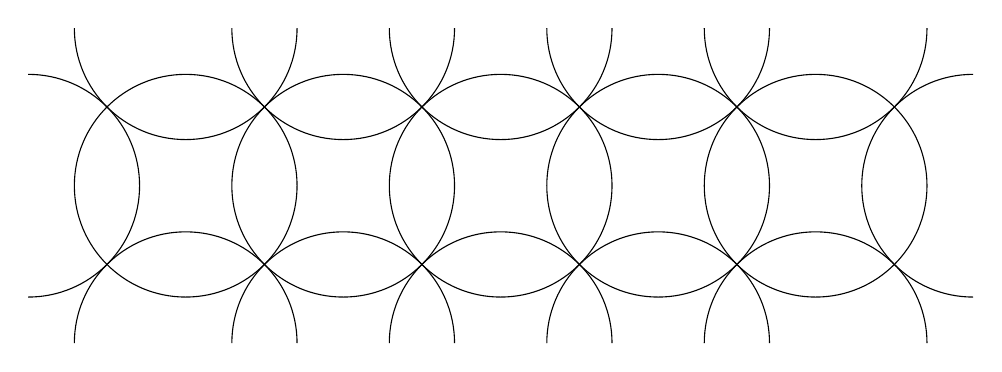
\begin{tikzpicture}
\draw (-2,-1.4142) arc [radius=1.4142, start angle=-90, end angle= 90];
\draw (10,-1.4142) arc [radius=1.4142, start angle=270, end angle= 90];
\foreach \x in {0,2,4,6,8}{
  \draw (\x,0) circle [radius=1.4142];
  \draw (-1.4142 + \x,-2) arc [radius=1.4142, start angle=180, end angle= 0];
  \draw (-1.4142 + \x,2) arc [radius=1.4142, start angle=-180, end angle= 0];
}
\end{tikzpicture}
\caption{A tiling of the plane created by overlapping circles, consisting of
digons and concave quadrilaterals with curved edges.}
\label{fig:circlesquare}
\end{figure}

An \textit{orientable} polyhedron is one where each face's vertices may be assigned a cyclic order such that each edge, say with vertices $a$ and $b$, has an order of $a$ to $b$ in one face and the reverse order $b$ to $a$ in the other. \cite{grunbaum94} A polyhedron that is not orientable is \textit{non-orientable}. All polyhedra with an odd Euler characteristic are non-orientable, e.g. the hemicuboctahedron. That said, all non-orientable polyhedra have an orientable double cover that is connected. (An orientable polyhedron also has an orientable double over, consisting of two disjoint copies of the original polyhedron.)

An \textit{achiral polyhedron} is one that has mirror symmetry:
a \textit{chiral polyhedron} is one that does not. Note that the particular
handedness of a chiral polyhedron is a quality of the realization, not the
underlying abstract polyhedron.
Also note that chirality depends on the space the polyhedron is embedded in:
polyhedra that are chiral in $\mathbb{R}^3$ are not in $\mathbb{R}^4$.

An \textit{acoptic polyhedron} is (loosely) a polyhedron that does not
self-intersect. \cite{grunbaum99} Its faces are simple polygons with straight
edges that do not self-intersect (although they may be concave). A
\textit{convex polyhedron} is an acoptic polyhedron that is convex: any line
between points on the surface of the polyhedron is contained in the interior of
the polyhedron. By Steinitz's theorem, the skeleton of every convex polyhedron
is a 3-vertex-connected planar graph. Furthermore, all convex polyhedra have a
realization such that each edge is tangent to the unit sphere, each face is
flat, and the centroid of the vertices lies at the origin.\cite{ziegler}
This is called the \textit{canonical realization}.

An \textit{operator on polyhedra} is simply a map $x : \mathcal{P} \to
\mathcal{P}$, where $\mathcal{P}$ is the set of polyhedra. We'll often apply
operators to a restricted set of polyhedra, e.g. convex polyhedra, orientable
polyhedra, or polyhedra with triangular faces. Sometimes we will look at maps
satisfying $x : \mathcal{X} \to \mathcal{Y}$ where $\mathcal{X}$ and
$\mathcal{Y}$ are different subsets of polyhedra: we will still call these
operators on polyhedra (instead of transformations). We'll use a calligraphic
typeface for sets of polyhedra or quasipolyhedra. The set of polyhedra without
digons or degree-2 vertices is here denoted $\mathcal{P}_3$, and the set of
polyhedra with 3-vertex-connected skeletons is $\mathcal{P}_{3v}$.

Some of these sets have additional structure, such as a specific coloring of
the vertices or faces. One fundamental distinction is between orientable and
non-orientable polyhedra. If a polyhedron is orientable, then there are two
choices of orientation to apply to it. We'll call the orientable polyhedra,
plus a choice of orientation, the \textit{oriented polyhedra}, and denote them
$\mathcal{P}^o$. Other subsets of polyhedra that are orientable will share this
superscript $o$ notation, so e.g. $\mathcal{P}^o_3$ is the set of orientable
polyhedra without digons or degree-2 vertices.

The set of polyhedra with even-sided faces is denoted $\mathcal{E}$. If also
orientable, ($\mathcal{E}^o$), the vertices of the polyhedron can be 2-colored.
The particular choice of coloring (out of the two possible colorings) is also
part of the additional structure of $\mathcal{E}^o$,
in addition to the orientation.

$\mathcal{W}$ is here defined as the set of polyhedra with only triangular
faces, such that the vertices of the polyhedron can be 3-colored. The faces of
a polyhedron in $\mathcal{W}^o$ can also be 2-colored. Such polyhedra are
important to Antiprism's implementation of many operations.

\section{Notable operations}

This section isn't a complete survey of operations on polyhedra. Some
operations have had ambiguous or changing definitions in the past, so going
through all that history would just muddy the waters. Instead, this section
summarizes some useful operators that motivate the discussion herein or will
be applied.

\subsection{Operations defined in Coxeter's Regular Polytopes}

In Coxeter's classic text \textit{Regular Polytopes}\cite{coxeter73},
he defines a handful of operations on regular polytopes:
\begin{itemize}
  \item The dual is defined in the usual way, compatible with how it was
  defined earlier in this text.
  \item Various forms of truncation are defined. The simple truncation is
  described by analogy with the polygonal case: cut off each corner of a
  polygon in such a way that the new polygon has vertices at the midpoint of
  each original edge. Other forms of truncation that retain part of the original
  edge are mentioned but not described. It is also commented that for regular
  polyhedra, the truncation is equivalent to the intersection
  of the (canonical realization of) the original polyhedra and its dual.
  \item An operation, partial truncation or alternation, is defined on regular
  polytopes with even-degree faces. Alternating vertices are cut off or
  retained. This results in digons for degree-4 faces,
  which are treated as edges.
  \item The snub operation (different than Conway's snub)
  is equivalent to simple truncation followed by alternation.
\end{itemize}

Coxeter's construction of simplexes can be cast in terms of abstract polyhedra.
Simply take the poset direct product of a number of copies of the unique
abstract polyhedron of rank 1 (a single point). The product of two points is an
edge: of three, a triangle, of four, a tetrahedron, and so on. This can be
thought of as a binary operation on simplexes, so e.g. the product of two edges
is a tetrahedron. (Also, suggestively, the $f$-polynomial of a direct product
of posets is the product of the $f$-polynomial of each poset.)

\subsection{Conway's operations}
Conway described a set of operations on polyhedra and a notation for describing
those operations, with the intent of creating a systematic naming scheme for
polyhedra.\cite{conway} He used a prefix notation, where the rightmost element
is a polyhedral seed and operators apply from right to left. Each operator is
assigned a letter and a name. So, for instance, $dO$ is the dual of a regular
octahedron (i.e. a cube), and $taO$ is a truncated ambo octahedron, more
commonly known as the truncated cuboctahedron. Conway's original set of
operations is denoted with the letters $abdegjkmost$: a full list of their
descriptions will be given in Appendix B. These operations are sufficient to
create all of the Archimedean and Catalan solids from the Platonic solids.
Others have defined more operations.
\cite{hart98}\cite{hart00}\cite{antiprism} In particular, Hart \cite{hart98}
defined $r$, which reverses the chirality of a polyhedra. The term "Conway
operator" is actually a little ambiguous: it may refer to Conway's original
set of operations, or an expanded set, or the general idea of notation
polyhedra by alphabetical prefixes.

Aside from $g, s, j$, and $a$, Conway's operations preserve the
symmetry of the resultant polyhedra. $g$ and $s$ are achiral, so
do not preserve mirror symmetry. $j$ and $a$ actually increase
the symmetry: in fact, the other 4 Platonic solids can be expressed
in terms of the tetrahedron $T$ using $j$ and $a$.

Some of Conway's operations can be expressed in terms of other operations:
$e=aa, o=jj, m=kj$, and $b=ta$, as well as the ones that are dual to each other.

Some Conway operators have an indexed form that indicates that only certain faces or
vertices are operated on. For instance, $k_i$ applies kis to faces with
$i$ sides, and $t_i$ truncates vertices of degree $i$.
Operations like this do not in general preserve the symmetry of the seed
polyhedron.

\subsection{Goldberg-Coxeter operations}
The Goldberg-Coxeter operation (GC operation) was defined by Deza and Dutour
\cite{dutour}, based on the Goldberg polyhedra, the viral capsid structure
defined by Coxeter \cite{coxeter71}, the geodesic domes of Buckminster Fuller,
and similar structures. Essentially it amounts to replacing the faces of a
polyhedra with a section from a grid of triangular or square faces, termed the
"master polygon" by Deza and Dutour. Here the operation on triangle-faced
polyhedra will be denoted $\Delta_{n,m}$, and on quadrilateral-faced polyhedra
$\Box_{n,m}$, where $n$ and $m$ are integers, $n > 0$, and $m \ge 0$.

$\Delta_{n,m}$ can be described using the triangular lattice over the
Eisenstein integers. It is useful for this operation to parameterize the
Eisenstein integers as $x = n + mu$ where $u = \frac{1}{2}(1 + i\sqrt 3) =
e^{\pi i/3}$, for reasons to be explained later. The master polygon is the
section of the grid contained in the triangle $0, x, xu$. It may also be useful
to identify an edge-centered section of the grid,
given by $0, x(2-u)/3, x, x(1+u)/3$.

$\Box_{n,m}$ can be described using the triangular lattice over the Gaussian
integers, $x = n + mi$ where $i = \sqrt{-1}$. The master polygon is contained
in $0,x,(x+i),xi$, and the edge-centered section is $0, x(1-i)/2, x, x(1+i)/2$.

Each operator has an invariant $g$, equivalent to $g = |x|^2$. For
$\Delta_{n,m}$, $g = n^2 + m^2$: for $\Box_{n,m}$, $g = n^2 + nm + m^2$. This
can be used to calculate the $f$-vector of the resulting polyhedron
based on the $f$-vector of the seed polyhedron. (The actual formula
will be shown later in a more general form.)

Two elements of the Eisenstein integers $x$ and $y$ are associates if
$y = u^k x$ for some integer $k$. Similarly, two elements of the Gaussian integers are
associates if $y = i^k x$ for some $k$. The associated element with $n>0$ and
$m\ge 0$ is the normal form. (We use the alternate definition for Eisenstein
integers so that the same definition for normal form applies to both operators.
This is also the traditional definition used by Goldberg polyhedra, geodesic
domes, viral capsids, etc.) Iff $n+mu$ is associated with $(a+bu)(c+du)$, then
$\Delta_{a,b}\Delta_{c,d} = \Delta_{n,m}$, and similarly for $\Box_{a,b}$.

Another consequence of the relationship between these operators and the
Eisenstein and Gausssian integers is that these operators are commutative and
associative: $\Delta_{a,b}\Delta_{c,d} = \Delta_{c,d}\Delta_{a,b}$, and
similarly for $\Box_{a,b}$. Furthermore, the Eisenstein and Gaussian integers
are Euclidean domains, which means elements of the domains can be factored
uniquely (if not irreducible), and there is a straightforward way to do so
using an extension of the Euclidean algorithm. (The invariant $g$ is the
Euclidean function in the Euclidean algorithm.) Therefore, it's straightforward
to reduce $\Delta_{n,m}$ and $\Box_{n,m}$ into other operators, in
and the irreducible operators correspond to Eisenstein or Gaussian primes.

These operators are divided into three classes.
\begin{itemize}
  \item Class I: $m = 0$, achiral
  \item Class II: $n = m$, achiral
  \item Class III: All others, chiral, requires orientable polyhedron.
\end{itemize}
All Class II operators can be reduced as
$\Delta_{n,n} = \Delta_{1,1}\Delta_{n,0}$, and possibly further (and similiarly
for $\Box_{n,n}$). In fact, $\Delta_{n,m}$ is reducible if $n \equiv m \mod 3$
(as $\Delta_{1,1}$ and some other $\Delta_{c,d}$), and $\Box_{n,m}$ is
reducible if $n \equiv m \mod 2$ (as $\Box_{1,1}$ and some other $\Box_{c,d}$).

When applied to the triangular tiling of the plane, $\Delta_{n,m}$ produces a
(possibly scaled and rotated) triangular tiling of the plane, regardless of
subscript. The same holds for $\Box_{n,m}$ and the quadrilateral tiling of the
plane.

\subsection{Operations in the software package Antiprism}

The software package Antiprism \cite{antiprism} includes a number of
applications that perform operations on polyhedra. (Among other things, it
contains an implementation of Conway operations in \texttt{conway}.) One
caveat: The file format used by antiprism, OFF, consists of a list of vertex
positions and a list of faces that references the list of vertices. This is
not a fully faithful representation of a polyhedra, as it does not contain
explicit incidence information. Any polyhedron whose abstract polyhedron is
not atomistic cannot be represented faithfully in Antiprism: e.g. polyhedra
with overlapping faces or digons. Digons are referred to as explicit edges by
antiprism.

Of particular interest is the application \texttt{wythoff}, in which a notation
for operations on polyhedra is introduced. Despite the name, the new notation
is much more flexible than Wythoff notation. \texttt{wythoff} automatically
applies Conway's meta operation to produce a polyhedron in $\mathcal{W}^o$. The
meta operation retains the original vertices and adds a vertex at the center of
each edge and each face. Respectively, these are labeled $V$, $E$, and $F$. If
a polyhedron is in $\mathcal{W}^o$ it can be used directly: the labeling of
vertices uses the same letters VEF. This is somewhat confusing since E and F no
longer relate to edges or faces, so alternately the vertices can be labeled
ABC. If applied to a non-orientable polyhedron, \texttt{wythoff} instead uses
the orientable double cover of the polyhedron.

For example, this is the string that it uses to implement Conway's kis
operation: \texttt{[F, V] 0\_1v1v, 1E}. The extended Wythoff notation comprises
two parts. The first part, in brackets, defines points on each triangular face
using barycentric coordinates. Each point is specified as \texttt{aVbEcF}, where
\texttt{a}, \texttt{b}, and \texttt{c} are numbers. If any of those are 1, the
number may be left off: if 0, the component may be left off. So in the above,
it defines two points, more explicitly as \texttt{0V0E1F} and \texttt{1V0E0F}:
a point at vertices labeled $F$, and a point at vertices labeled $V$.

The second part defines faces as paths between these points. A \texttt{+},
\texttt{-}, or \texttt{*} at the start of a path denotes which triangle to
start with: if none, then \texttt{+} is assumed. An underscore indicates
remaining on the same triangle. A lowercase \texttt{v}, \texttt{e}, or
\texttt{f} indicates that the path crosses the edge opposite of the vertex
labelled $V$, $E$, or $F$. An uppercase \texttt{V}, \texttt{E}, or \texttt{F}
indicates a rotation by two triangles about the vertex labeled $V$, $E$, or $F$:
explicitly, these are shorthands for \texttt{ef}, \texttt{fv}, and \texttt{ve}
respectively. The first path starts at point 0 on + triangles, moves to point 1
on the same triangle, then moves over the edge opposite $V$ to point 1 on
that triangle. It then moves back over the edge and completes the path at 0
on the original triangle. (The second produces an explicit edge, and is needed
so that the operation produces a polyhedron when applied directly to a
polyhedron in $\mathcal{W}^o$.)

This notation is capable of representing many operations on polyhedra,
including all of Conway's operators. (In fact the current version of
\texttt{conway} uses \texttt{wythoff} to implement the operators.) Notation to
create the regular hemihedra from the Platonic solids exists, as does notation
to create hollowed-out, da Vinci-style renderings of polyhedra. It can be
applied to partial tilings of the plane or partial polyhedra, although it more
or less skips the edges that are adjacent to less than 2 faces. It may also
produce quasipolyhedra: in fact, care should be taken to make sure that the
notation produces a polyhedron in all cases, not just when applied with the
meta operation.

\section{Smoothing}

Digons can be present in a faithful realization of a polyhedron, such as in
Figure \ref{fig:circlesquare}, or spherical hosohedra. However, many
definitions or subsets of polyhedra exclude digons. (For instance, Gr\"unbaum
excludes digons in \cite{grunbaum03}.) Degree-2 vertices are also problematic,
being dual to digons. These elements can be eliminated in a systematic manner.
We define a smoothing operator, $\$$, that transforms digons into single edges
and handles degree-2 vertices by removing that vertex and merging the vertex's
incident edges, as depicted in figure \ref{fig:smooth}. In graph-theoretic
terms, degree-2 vertices are transformed by contracting one of the edges it
connects to, and digons are transformed by collapsing their edges into one,
which is the equivalent act on the dual graph. \cite{gross} Antiprism
effectively smooths digons automatically by treating them as "explicit edges".

\begin{figure}
\begin{tikzpicture}
\draw (0,0) -- (0,2);
\draw (0,1) -- (3,1);
\draw (3,0) -- (3,2);
\draw[fill] (0,1) circle [radius=0.05];
\draw[fill] (1.5,1) circle [radius=0.05];
\draw[fill] (3,1) circle [radius=0.05];

\draw (4.5,0) -- (4.5,2);
\draw (4.5,1) to [out=45,in=135]  (7.5,1);
\draw (4.5,1) to [out=-45,in=-135]  (7.5,1);
\draw (7.5,0) -- (7.5,2);
\draw[fill] (4.5,1) circle [radius=0.05];
\draw[fill] (7.5,1) circle [radius=0.05];

\draw (9,0) -- (9,2);
\draw (9,1) -- (12,1);
\draw (12,0) -- (12,2);
\draw[fill] (9,1) circle [radius=0.05];
\draw[fill] (12,1) circle [radius=0.05];
\end{tikzpicture}

\caption{Depiction of smoothing operator $\$$. a) a degree-2 vertex b) digon c)
        smoothed result when applied to either.}
\label{fig:smooth}
\end{figure}

Smoothing a single digon removes 1 face and 1 edge from the polyhedron.
Smoothing a single degree-2 vertex removes 1 vertex and 1 edge.
If $f_p$ is the f-vector of a polyhedron, then $f_{\$p} \le f_p$, where the
inequality holds pairwise.

\begin{figure}
\begin{tikzpicture}
\draw (0,0) -- (0,2);
\draw (0,1) -- (1,1);
\draw (1,1) to [out=45,in=135]  (2,1);
\draw (1,1) to [out=-45,in=-135]  (2,1);
\draw (2,1) -- (3,1);
\draw (3,0) -- (3,2);
\draw[fill] (0,1) circle [radius=0.05];
\draw[fill] (1,1) circle [radius=0.05];
\draw[fill] (2,1) circle [radius=0.05];
\draw[fill] (3,1) circle [radius=0.05];

\draw [->] (3.5,1) -- (4,1);

\draw (4.5,0) -- (4.5,2);
\draw (4.5,1) -- (7.5,1);
\draw (7.5,0) -- (7.5,2);
\draw[fill] (4.5,1) circle [radius=0.05];
\draw[fill] (5.5,1) circle [radius=0.05];
\draw[fill] (6.5,1) circle [radius=0.05];
\draw[fill] (7.5,1) circle [radius=0.05];

\draw [->] (8,1) -- (8.5,1);

\draw (9,0) -- (9,2);
\draw (9,1) -- (12,1);
\draw (12,0) -- (12,2);
\draw[fill] (9,1) circle [radius=0.05];
\draw[fill] (12,1) circle [radius=0.05];
\end{tikzpicture}

\caption{A multi-step smoothing series.}
\label{fig:multismooth}
\end{figure}

Conceptual complications arise when a polyhedron contains multiple digons or
2-vertices incident to one another. There is some choice in which element to
start on, and degree-2 elements may be adjacent to one another. A single
smoothing step may create other degree-2 elements, as depicted in Figure
\ref{fig:multismooth}. It can be shown that with repeated reduction of single
elements, the polyhedron eventually reaches a state where it has no degree-2
features. We choose to define $\$$ so that it produces a polyhedron where all
degree-2 features have been removed. There may also be other ways to smooth a
particular configuration involving a degree-2 feature that may have other
benefits, e.g. Figure \ref{fig:weirdo},
but $\$$ is the minimum-effort way to remove the degree-2 features.

\begin{figure}
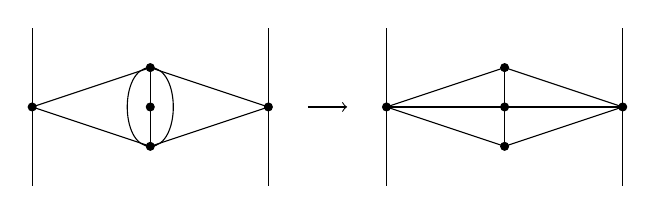
\begin{tikzpicture}
  \draw (0,0) -- (0,2);
  \draw (0,1) -- (1.5,1.5) -- (3,1);
  \draw (0,1) -- (1.5,0.5) -- (3,1);
  \draw (1.5,0.5) -- (1.5,1.5);
  \draw (1.5,0.5) to [out=0,in=0] (1.5,1.5);
  \draw (1.5,0.5) to [out=180,in=180] (1.5,1.5);
  \draw (3,0) -- (3,2);
  \draw[fill] (0,1) circle [radius=0.05];
  \draw[fill] (1.5,1.5) circle [radius=0.05];
  \draw[fill] (1.5,1) circle [radius=0.05];
  \draw[fill] (1.5,0.5) circle [radius=0.05];
  \draw[fill] (3,1) circle [radius=0.05];

  \draw [->] (3.5,1) -- (4,1);

  \draw (4.5,0) -- (4.5,2);
  \draw (4.5,1) -- (6,1.5) -- (7.5,1);
  \draw (4.5,1) -- (6,0.5) -- (7.5,1);
  \draw (4.5,1) -- (7.5,1);
  \draw (6,0.5) -- (6,1.5);
  \draw (7.5,0) -- (7.5,2);
  \draw[fill] (4.5,1) circle [radius=0.05];
  \draw[fill] (6,1.5) circle [radius=0.05];
  \draw[fill] (6,1) circle [radius=0.05];
  \draw[fill] (6,0.5) circle [radius=0.05];
  \draw[fill] (7.5,1) circle [radius=0.05];
\end{tikzpicture}

\caption{A more complicated degree-2 feature and its surroundings,
and a particular way it admits a smoothing that preserves the count of
elements.}
\label{fig:weirdo}
\end{figure}

In special circumstances $\$$ may produce quasipolyhedra. For instance, the
result for any spherical hosohedron or spherical dihedron is the digonal
hosohedron or monogonal dihedron, respecetively. It may be helpful to define
the operator such that it returns a proper polyhedra,
stopping before it produces a quasipolyhedron.
This ambiguity will not affect the rest of this text.

With some odd exceptions (those in the last paragraph), the smoothing operator
$\$$ produces polyhedra where the minimum vertex and face degree is 3. Since
the original polyhedron was required to be connected, this also means that the
polyhedron has a 3-edge-connected skeleton. This is necessary but not
sufficient in order to have a 3-vertex-connected skeleton (which, if the graph
is also planar, makes it the skeleton of a convex polyhedron). One feature
preventing a 3-edge-connected skeleton from being a 3-vertex-connected skeleton
can be seen on the left of Figure \ref{fig:pound}. In general, if a
3-edge-connected graph has any subgraphs that can be reduced to a digon or
degree-2 vertex by edge contraction, those are responsible for the graph not
being a 3-vertex-connected graph. So, we introduce an operator that does that
edge contraction and then removes the resulting degree-2 feature, and call it
\textit{pound}, denoted $\pounds$. (The name is by analogy with pounding out
the dents in a metal object to make it convex, and using a currency symbol
makes it similar to $\$$.) That said, polyhedra with such features and
operators that produce them are interesting in ways we'll get to later.

\begin{figure}
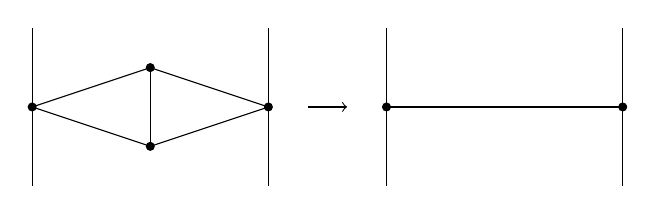
\begin{tikzpicture}
\draw (0,0) -- (0,2);
\draw (0,1) -- (1.5,1.5) -- (3,1);
\draw (0,1) -- (1.5,0.5) -- (3,1);
\draw (1.5,0.5) -- (1.5,1.5);
\draw (3,0) -- (3,2);
\draw[fill] (0,1) circle [radius=0.05];
\draw[fill] (1.5,1.5) circle [radius=0.05];
\draw[fill] (1.5,0.5) circle [radius=0.05];
\draw[fill] (3,1) circle [radius=0.05];

\draw [->] (3.5,1) -- (4,1);

\draw (4.5,0) -- (4.5,2);
\draw (4.5,1) --  (7.5,1);
\draw (7.5,0) -- (7.5,2);
\draw[fill] (4.5,1) circle [radius=0.05];
\draw[fill] (7.5,1) circle [radius=0.05];
\end{tikzpicture}

\caption{Depiction of pound operator $\pounds$.}
\label{fig:pound}
\end{figure}

\section{Edge-replacement operations}
From this point, the discussion will exist in an uncomfortable middle ground.
We will usually only be concerned with the combinatorial or topological
structure of the polyhedron, but we still need to make reference to the ambient
space. For instance, a \textit{face center} as used here need not be at any
exact center of the face, or even really on the face, but the most intuitive
way to talk about it is to put it at some sort of center on the face. When we
talk about equality of operators, we mean it in the topological and combinatorial sense.

In \cite{brinkmann}, two sets of operations on polyhedra are defined: local
symmetry-preserving operations (LSP), on $\mathcal{P}$, and local operations
that preserve orientation-preserving symmetries (LOPSP), on $\mathcal{P}^o$.
\textit{Symmetry-preserving} means that the symmetry group of the seed
polyhedron is the same as or a subgroup of the symmetry group of the result
polyhedron. All of Conway's original operators are LSPs,
except for gyro ($g$) and snub ($s$), which are LOPSPs. If the seed
polyhedron's faces have an orientation, such that the seed already doesn't
have mirror symmetry, then LOPSP are symmetry-preserving in the same sense as
LSPs. $r$ is not an LOPSP, since it reverses the orientation of an oriented
polyhedron, but $rxr$ is an LOPSP if $x$ is. If $x$ is an LSP, then $r$ is
equivalent to $S$: $rx = xr = rxr = x$, at least in combinatorial terms.

For LSPs and LOPSPs, the ratio of edges in the result polyhedron to the seed
polyhedron is an invariant of the operator, and is always a positive integer.
This is termed the \textit{inflation rate} by \cite{brinkmann},
and denoted $g$ (not to be confused with the operator).
It can also be termed the \textit{edge multiplier}.

\begin{figure}
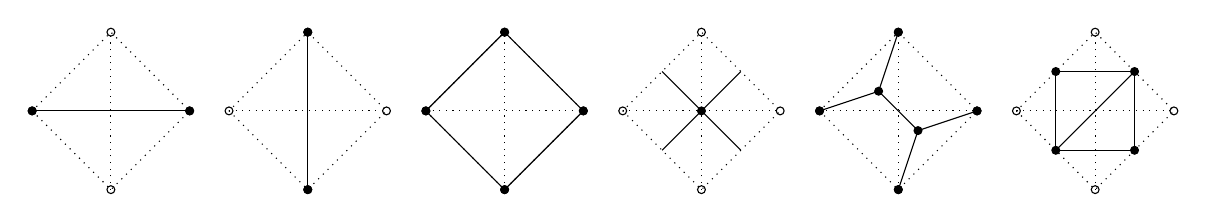
\begin{tikzpicture}
    \pic at (0,0) {chamber4};
  \draw (0,1) -- (2,1);
  \draw[fill] (0,1) circle [radius=0.05];
  \draw[fill] (2,1) circle [radius=0.05];

  \pic at (2.5,0) {chamber4};
\draw (3.5,0) -- (3.5,2);
\draw[fill] (3.5,0) circle [radius=0.05];
\draw[fill] (3.5,2) circle [radius=0.05];

\pic at (5,0) {chamber4};
\draw (5,1) -- (6,0) -- (7,1) -- (6,2) -- (5,1);
\draw[fill] (5,1) circle [radius=0.05];
\draw[fill] (6,0) circle [radius=0.05];
\draw[fill] (7,1) circle [radius=0.05];
\draw[fill] (6,2) circle [radius=0.05];

\pic at (7.5,0) {chamber4};
\draw (8,0.5) -- (9,1.5);
\draw (9,0.5) -- (8,1.5);
\draw[fill] (8.5,1) circle [radius=0.05];

\pic at (10,0) {chamber4};
\draw (10,1) -- (10.75,1.25) -- (11,2);
\draw (12,1) -- (11.25,0.75) -- (11,0);
\draw (10.75,1.25) -- (11.25,0.75);
\draw[fill] (11,0) circle [radius=0.05];
\draw[fill] (11,2) circle [radius=0.05];
\draw[fill] (10,1) circle [radius=0.05];
\draw[fill] (12,1) circle [radius=0.05];
\draw[fill] (10.75,1.25) circle [radius=0.05];
\draw[fill] (11.25,0.75) circle [radius=0.05];

  \pic at (12.5,0) {chamber4};
\draw (13,1.5) -- (14,1.5) -- (14,0.5) -- (13,0.5) -- (13,1.5);
\draw (14,1.5) -- (13,0.5);
\draw[fill] (13,1.5) circle [radius=0.05];
\draw[fill] (14,1.5) circle [radius=0.05];
\draw[fill] (14,0.5) circle [radius=0.05];
\draw[fill] (13,0.5) circle [radius=0.05];
\end{tikzpicture}

\caption{Edge-centered diagram of EROs (LSPs and LOPSPs). From right to left:
Seed ($S$), dual ($d$), join ($j$), ambo ($a$), gyro ($g$), snub ($s$).}
\label{fig:edgecentered}
\end{figure}

Both LSPs and LOPSPs can be depicted in an edge-centered diagram like in Figure
\ref{fig:edgecentered}. The idea is quadrilaterals can be identified on a
polyhedron that contain each edge and have vertices going from one vertex of
that edge, the face center to one side of the edge, the other vertex of the
edge, and the face center to the other side of the edge. Then, that
quadrilateral can be replaced with these edge-centered diagrams. The original
vertices of the seed polyhedron are the point of the quadrilateral on the left
and right of the diagram, while the original face centers are those on the top
and bottom. Vertices are a filled dot, while face centers that are retained as
a face are an open dot. Because LSPs and LOPSPs can be depicted like this, and
since \cite{brinkmann} didn't introduce a term for it, we call the two sets of
operators together \textit{edge-replacement operators}, or \textit{ERO}s.

Edge-centered diagrams show four chambers, two to each side of the seed edge.
For LOPSPs, the chambers of the top 2 chambers are a one-half-turn rotation of
the bottom two. For LSPs, the chambers are all reflections of each other over
the dotted lines. There is some redundancy built into these diagrams. We might
think back to our explanation of \texttt{wythoff} and how it generally starts
with a meta operation $m$, and note that the $m$'s edge-centered diagram would
create a line over each dotted line, and wonder if we can create these
operators as a composition of $m$ and some other operator from
$\mathcal{W}$ to $\mathcal{P}$ or $\mathcal{W}^o$ to $\mathcal{P}^o$.

The last statement is true, in a more complicated form. Figure
\ref{fig:facediagram} depicts face diagrams for operators that can be used to
produce the operators from Figure \ref{fig:edgecentered}. The first thing to
note is that an edge cannot pass through the corners of the face diagram
without a vertex at that corner. If it could, there could be edges connecting
3 or more vertices, which is forbidden. The second is that we can permute the
vertices of these face diagrams to produce new operators. Here we introduce an
operator, $@$, to represent that permutation. $@_{ABC}$ maps A, B, and C
to V, E and F in the seed polyhedron produced by $m$. (In general, $@$ acts on
the vertex coloring of polyhedra in $\mathcal{W}$.) The third is that the $m$
operator always produces a vertex of degree 4 at the center of each edge.

\begin{figure}
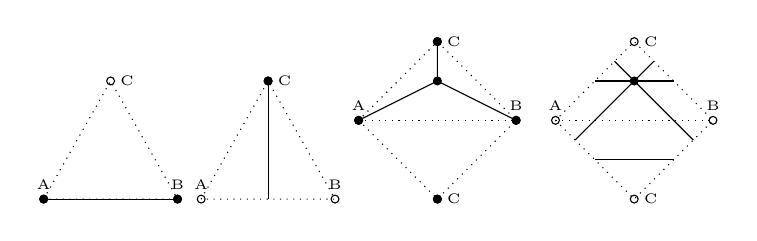
\begin{tikzpicture}
  \pic at (0,0) {chamber1};
\draw (1.7, 0) -- (0, 0);
\draw[fill] (0, 0) circle [radius=0.05];
\draw[fill] (1.7, 0) circle [radius=0.05];

\pic at (2,0) {chamber1};
\draw (2.85,0) -- (2.85,1.5);
\draw[fill] (2.85, 1.5) circle [radius=0.05];

\pic at (4,0) {chamber2};
  \draw[fill] (5,1.5) circle [radius=0.05];
  \draw[fill] (5,0) circle [radius=0.05];
  \draw[fill] (5,2) circle [radius=0.05];
  \draw[fill] (4,1) circle [radius=0.05];
  \draw[fill] (6,1) circle [radius=0.05];
  \draw (5,2) -- (5,1.5) -- (4,1);
  \draw (5,1.5) -- (6,1);

\pic at (6.5,0) {chamber2};
  \draw[fill] (7.5,1.5) circle [radius=0.05];
  \draw (7,1.5) -- (8,1.5);
  \draw (7,0.5) -- (8,0.5);
  \draw (7.25,1.75) -- (8.25,0.75);
  \draw (7.75,1.75) -- (6.75,0.75);
\end{tikzpicture}

\caption{Face diagram of some operators.}
\label{fig:facediagram}
\end{figure}

Let $x$ be the operator in the first face diagram from Figure
\ref{fig:facediagram}. $x@m$ produces different operators, depending on the
subscript to $@$. ACB and BCA produce the join operator $j$. ABC and BAC
produce something that is almost, but not quite the identity operator $S$,
while CAB and CBA almost produce the dual operator $d$. The degree 4 vertex at
the edge center has had its order halved, to a degree 2 vertex. Applying the
smoothing operator $\$$ will remove that vertex. So it makes sense, if degree-2
elements are undesirable, to create operators as $\$x@m$.

If $y$ is operator in the second face diagram from Figure \ref{fig:facediagram},
then $\$x@m$ is $d$ for ABC and BAC, $S$ for CAB and CBA, and $a$ for ACB and
BCA. Note that we have two different expressions for $S$ and $d$ now. For the
expression in terms of $x$, degree-2 vertices were removed, and in terms of
$y$, digons were removed.
At most six operators can arise from the different permutations of an operator:
the aforementioned have some the same due to symmetry.

For LOPSPs, the situation is a little more complicated by keeping track of
orientations. See the last two face diagrams in Figure \ref{fig:facediagram},
which correspond to $g$ and $s$. Starting with A and travelling
counterclockwise in each triangle, the first triangle is ABC, while the second
is ACB. Thus, the upper triangle is applied to even-permutation faces from the
seed in $\mathcal{W}^o$, while the lower triangle is applied to odd-permutation
faces. (Also, note that for these operators,
all even permutations result in the same operator for these face diagrams,
and all odd permutations result in the chiral pair of that operator.) There is
some flexibility in where vertices can be placed in the face diagram while
representing a (topologically) equivalent operator: they can be moved onto a
seed edge, or to the other face. Thus, some of the operations in this text may
not have exactly the same appearance as in other publications.

Given what we've discussed so far, it is easily shown that all EROs can be
expressed as $y = \$x@m$ for some $x$, where $y$ operates on $\mathcal{P}_3$.
(If the seed polyhedron contains degree-2 elements, those will also be reduced
by the $\$$ term, so to exclude that case we restrict it to polyhedra without
such elements. It's possible that there is a definition of $\$$ or grouping
of operators that would allow for extension to all polyhedra.) If the edge
multiplier $g$ for $y$ is even, there is an $x$ such that $y = x@m$, with no
smoothing step needed. If $g$ is odd, then there are at least two $x$
satisfying $y = \$x@m$, one which will have a digon removed and one which will
have a degree-2 vertex removed. (There may be further relations where more than
one digon or degree-2 vertex is removed.) Relatedly, if $g$ is even it either
has a vertex or a face at the center of its edge-centered diagram:
if odd, it has an edge there.

The aforementioned also makes it very easy to describe $yd$ given $y$.
Remember that the dual operator interchanges vertices and faces. Therefore,
$md$ produces a polyhedra with V and F in opposite places. In a formula,
$\$xmd = \$x@_{CBA}d$. Thus, the edge-centered diagram for $yd$ is that for
$y$, rotated one-quarter-turn.

Borrowing an idea from ring theory, we refer to $d$ (dual), $S$ (seed,
identity) as the units of the EROs, and operators that are related by $d$ are
called associates. ($r$ is a little odd and will be left out.) At most 4
distinct operators can be associated with each other, corresponding to $x$,
$xd$, $dx$, and $dxd$. Conway's operators are associated as so:
\begin{itemize}
  \item $j=jd, a=dj=djd$
  \item $k, t=dkd$ (as well as $n=kd$ and $z=dk$)
  \item $o=od, e=do=dod$
  \item $g, s=dgd$ (as well as $rgr=gd$ and $rsr=sd$)
  \item $m=md, b=dm=dmd$
\end{itemize}
Appendix B lists all named operators with their associates.

We'll call operations on polyhedra that share their
operator on $\mathcal{W}$ or the dual of $\mathcal{W}$ as a \textit{cohort}. If
operators are associated, they share a cohort. There are at most 12 distinct
operators in a cohort. Appendix C lists all named operators and their cohort.

As a final note, EROs allow us to extend the Goldberg-Coxeter operations
$\Box_{n,m}$ and $\Delta_{n,m}$ to faces with any number of sides. We simply
have to identify the edge-centered diagram for EROs. The vertices of this
quadrilateral were given in the earlier section on GC operations. These
operators retain the same commutation and factoring properties in this
extension.

\section{Alternating EROs}
Recall that $m = kj$, so $y = \$x@m = \$x@kj$. $m: \mathcal{P} \to
\mathcal{W}$, as mentioned earlier, and $j: \mathcal{P} \to \mathcal{E}$, since
join produces only quadrilateral faces. As well, when $k$'s seed is in
$\mathcal{E}$, its result is in $\mathcal{W}$: this is true in general, not
just for the quadrilaterals $j$ produces. Combining this information leads us
to operators of the form $\$x@k: \mathcal{E} \to \mathcal{P}$. We call these
\textit{Vertex-Alternating EROs}, or \textit{VAEROs}. They have edge-centered
diagrams like EROs, but without the vertical center line. The leftmost corner
represents one color of vertex, and the rightmost represents another, while the
top and bottom still represent face centers. Notice that the orientation of
the diagram matters: if you have a diagram from $-$ to $+$, flip it one half
turn to get the diagram from $+$ to $-$. The similiar case for dual polyhedra
would be called \textit{Face-Alternating EROs}, or \textit{FAEROs}. Both taken
together are \textit{Alternating EROs} or \textit{AEROs}.

Coxeter's alternation operation $h$ is an VAERO. Let $x$ be the first face
diagram from Figure \ref{fig:facediagram}, then $\$x@_{ACB}k = h$. The inner
component $x@_{ACB}k$ creates degree-2 vertices where the seed polyhedron had
quadrilateral faces. Like with EROs, there is another $x$ that would create
digons instead. While the inner component has an inflation rate $g=1$,
this is not necessarily true for $h$ itself, since faces with 4 sides don't
exist in any fixed ratio for an arbitrary polyhedron in $\mathcal{E}$.

The join operator $j$ has a similar relation with duals as $m$. $j$ creates
vertices at the vertices and faces of the seed polyhedron, which implies a
2-coloring of the vertices. In $jd$, the same vertices are created, but their
correspondence to the vertices and faces of the seed is reversed. We can expand
the $@$ notation to apply to 2-colored vertices as well: $jd = @j$. Since there
are only two possible colorings, we don't need a subscript, and $@^2 = S$.
Furthermore, we can use the relation with $m$ from earlier: $md = @_{CBA}m =
kjd = k@j$, so we define $k@ = @_{CBA}k$.

This idea leads one to a possible edge-centered diagram method to construct
operators like $t_n$, truncation of vertices of degree $n$. Create three
edge-centered diagrams, one for edges between vertices of degree not equal to
$n$, one for edges between vertices of degree $n$, and one for edges with one
vertex of degree $n$ and one that is not. (Respectively, the first and second
would just be the diagrams for $S$ and $t$, and the last would look like $t$ or
$a$ on the left side and $S$ on the right.) Then use these diagrams to replace
their respective edges. A similar method could be used to handle partial
polyhedra: define an edge-centered diagram for edges where 2 faces meet, and
for edges adjacent to only 1 face.

\section{Other operations}

Technically, LSPs and LOPSPs as defined in \cite{brinkmann} are operators on
$\mathcal{P}_{3v}$. That excludes any operator that creates digons or degree-2
vertices, as well as any operator that creates the kind of features that
$\pounds$ removes, such as the Lozenge operator. It also excludes $r$,
as we mentioned earlier.

Some operators that do not preserve the topology of the seed polyhedron can be
described as EROs. \texttt{leonardo} in Antiprism creates attractive
hollowed-out polyhedra from seed polyhedra. The particular operation of
\texttt{leonardo} can't be performed in \texttt{wythoff}, but a similar one can
with the input string \texttt{[V, VF] 0\_1v1\_0v, 1v1f, 1V}. We call this the
\textit{Hollow} operation. The resulting polyhedron is acoptic if the seed has
positive curvature everywhere. If the seed had Euler characteristic 2 (genus
0), the result has Euler characteristic $4-2f$ (genus ($f-1$)). One could also
create operators that add arbitrary numbers of holes per edge. (Operators that
add cross-caps, e.g. based on a self-intersecting polyhedron with Euler
characteristic 1 such as the tetrahemihexahedron, may be possible. Such
operators probably have more theoretical uses than aesthetic or practical
ones, and their result would be hard to realize faithfully.)

It can help to understand operators like the Hollow operation by considering
two disjoint copies of the seed polyhedra that are then stitched together. We
define an operator, \textit{$n$-copy}, as the operator that creates $n$
disjoint copies of the seed. That said, the result of this operator is not a
polyhedron (it's multiple polyhedra), and it is ambiguous how to represent it
as a poset (specifically the maximal and minimal elements).

If we want to get even more abstract, we can think of these more general
topological operators as having the structure of a $\mathbb{N}$-module over a
semiring, where addition is the disjoint union of polyhedra, multiplication is
composition of operators, and a coefficient from $\mathbb{N} = {0, 1, ...}$
represents creating disjoint copies of a polyhedron. Then, the module has an
obvious homomorphism with the 3x3 matrices over $\mathbb{N}$.

\section{Invariants of EROs}
We already mentioned the inflation factor for EROs. \cite{brinkmann}
Expanding on that, many operations act on the $f$-vector as a linear operator.
Where $x$ is the operator, then the linear operator can be described with a
matrix:
\begin{equation}
  M_x = \begin{bmatrix}
  a & b & c \\
  d & g & h \\
  a' & b' & c' \end{bmatrix}
\end{equation}
If $x$ is an ERO, then $d = h= 0$. If $x$ perserves the Euler characteristic,
then the vector $(1,-1,1)$ is a left eigenvector of $M_x$ with eigenvalue $1$.
(Explicitly, $a + a' = d + 1$, $c+ c' = h+1$, and $b + b' + 1 = g$).

Some operators can also be expressed as an infinite linear operator $L_x$ on
the values $v_i$, $e$, and $f_i$: vertices of degree $i$, edges, and faces with $i$ sides, respectively. In particular, EROs take this form:
\begin{equation}
  \begin{split}
  E & = ge \\
  V_i & = a v_{i/k} + e b_i + c f_{i/\ell} \\
  F_i & = a' v_{i/k} + e b'_i + c' f_{i/\ell}
  \end{split}
\end{equation}
$v_i$, $e$, and $f_i$ are the input to the operator and $V_i, E$, and $F_i$ are
the result. $a, a', c,$ and $c'$ are either 0 or 1 if the Euler characteristic
is preserved. $g$ is a positive integer, all $b_i$ and $b'_i$ are nonnegative
integers, and $k$ and $\ell$ are positive integers.
$\sum b_i = b$ and $\sum b'_i = b'$. The subscripted
values like $v_{i/k}$ should be interpreted as 0 if $i/k$ is not an integer.

$L_x$ and $M_x$ for an ERO can be determined by counting elements off the
edge-centered diagram. Step by step:
\begin{itemize}
\item Seed vertices are either retained or converted into faces centered on that
  vertex. (Other options are precluded by symmetry). Let $a = 1$ if the
  seed vertices are retained, and 0 otherwise. Also, the degree of the vertex
  or face is either the same as the seed vertex, or a multiple of it;
  let $k$ be that multiple.
\item Seed face centers are either retained (possibly of in a smaller face) or
  converted into vertices. (Again, other options are precluded by symmetry).
  Let $c = 0$ if the seed faces are retained, and 1 otherwise. Let
  $\ell$ serve a similar role as $k$ above: the degree of the vertex
  or face corresponding to the seed face center is $k$ times the degree of
  the seed vertex.
\item Except for the faces or vertices corresponding to the seed vertices and face
  centers, the added elements are in proportion to to the number of edges in the
  seed. $g$ is the count of added edges (the edge multiplier or inflation
  rate), $b_i$ is the number of vertices of degree $i$ added, and
  $b'_i$ is the number of faces of degree $i$ added.
\end{itemize}
Count elements lying on or crossing the outer edge of the chamber structure as
half. It may help to draw an adjacent chamber, particularly when determining
the number of sides on a face.

Applying the handshake lemma to the skeleton graph of the polyhedron and its dual gives relations between the values for EROs:
\begin{equation}
  \begin{split}
   2g &= 2ak + 2c\ell + \sum i b_i \\
   2g &= 2a'k + 2c'\ell + \sum i b'_i
 \end{split}
\end{equation}
For Euler-characteristic preserving operations, these relations can be
manipulated into the form
\begin{equation}
  2k + 2\ell - 4 = \sum (4-i) (b_i + b'_i),
\end{equation}
which is interesting because it eliminates $g$, $a$ and $c$,
and because it suggests that features with degree 5 or more exist
in balance with features of degree 3 (triangles and degree-3 vertices),
and that in some sense degree 4 features come ``for free''.

With these relations, and the assumption that there are no degree 2 features
and therefore $i \ge 3$, a series of inequalities can be derived for EROs:
\begin{equation}
  \begin{split}
  g + 1 \le 2a + 3b + 2c \le 2g \\
  2k + 2\ell \le g + 3 \\
  0 \le 2k + 2\ell - 4 \le b_3 + b'_3 \\
  \end{split}
\end{equation}
Note that these inequalities are only necessary, not sufficient. For instance,
$g=4, a=1, c=0, b_4 = 1, b'_3=2, k=2, \ell=1$ satisfies the relations, but
doesn't appear to correspond to any ERO. Furthermore, the Lozenge operator
satisfies the relations.

It can be demonstrated that $M_{xy} = M_{x}M_{y}$ and $L_{xy} = L_{x}L_{y}$.
The expansion factor $g$ for the operator $xy$ is the product of the $g$
invariants for operators $x$ and $y$. It can also be seen that $a, a', c, c'$
form their own linear system, a submatrix of $M_x$: let $\Lambda_x =
\begin{bmatrix} a & c \\ a' & c' \end{bmatrix}$, then $\Lambda_{xy} = \Lambda_x
\Lambda_y$. $\Lambda_x$ represents the effect of the operator on the seed
faces and vertices. By cofactor expansion, $\det (M_x) = g \det (\Lambda_x)$.
$\Lambda_x$ has a determinant of $-1, 0$, or $1$. (In fact, $\Lambda_x$ has two
eigenvalues, one of which is always 1, and one of which may be -1, 0, or 1.
$M_x$ has three eigenvalues: two it shares with $\Lambda_x$, and one is $g$.)
The dual operator has $\det (M_d) = \det (\Lambda_d) = -1$, and it is easy to
see that of the four possible $\Lambda_x$, the two with determinant 0 are
related by the dual operator, and the two with determinant $\pm 1$ are related
by the dual operator. With that motivation, we define the \textit{Type} of the
operator as the absolute value of the determinant of $\Lambda_x$.

For EROs, the parity of the invariants $g$ and $b$ also describe the center of the chamber structure.
In particular, an ERO with both $g$ and $b$ odd is not possible.
\begin{itemize}
  \item $g$ even, $b$ even: A face with even degree lies at the center.
  \item $g$ even, $b$ odd: A vertex with even degree lies at the center.
  \item $g$ odd, $b$ even: An edge crosses the center.
  \item $g$ odd, $b$ odd: Excluded by symmetry.
\end{itemize}

$\Lambda_x$ can be used to prove that there are no EROs such that
$x = dx$ or $rxr = dx$. Other invariants can be used to prove the following.
Let $x$ be an ERO. If $rxr=xd$, $x$ has type 0. (Remember that $rxr = x$ if
$x$ is an LSP.) If $x=dxd$, $x$ is type 1, $g$ is odd, $b=b'$, and $b$ and
$b'$ are even. There are no LOPSPs $x$ with
$rxr = dxd$ or $x=xd$: either $x = dxd$, $rxr = xd$, or neither.
Unfortunately, no invariant for chirality has been discovered so far, either
to distinguish LSPs from LOPSPs or to distinguish the two parts of a chiral
pair of LOPSPs. The relationship with operators and chirality is complicated:
two chiral operators may produce another chiral operator (e.g.
$p^2 = \Box_{3,4}, g^2$) or an achiral operator ($prpr = \Box_{5,0}$).

EROs form a monoid (a group without inverses, or a semigroup with identity).
We have derived here a series of monoid homomorphisms, as
$x \to L_x \to M_x \to (g, \Lambda_x)$. None of these homomorphisms are
injections: there are certain $L_x$ or $M_x$ that correspond to more than one
EROs. Examples for $M_x$ are easy to come by: where $n = kd$, $M_k = M_n$. For
an example where the operators are not related by duality, $M_l = M_p$. For
$L_x$, $L_{prpr} = L_{pp}$ but $prpr = \Box_{5,0}$ is not the same as $p^2 =
\Box_{3,4}$ (one's chiral, one's not). For the Waffle operator, $W \ne Wd$,
but $L_W = L_{Wd}$. A general counterexample would be operators with
sufficiently large $g$ based on $\Box_{n,m}$, with a single square face (not
touching the seed vertices or face centers) divided into two triangles: the
counts of vertices of each degree, faces of each degree, and edges would be
the same no matter which faces was chosen, but the operators would be
different. With this construction, it is possible (with a sufficiently large
$g$) to create arbitrarily large sets of operators with the same invariants.

\section{Invariants of other operators}
Some VAEROs have a 4x3 matrix form from $v^+, v^-, e, f$ to $v, e, f$, where
$v^+, v^-$ are the counts of vertices of one color or the other. The matrix takes
this form:

\begin{equation}
  M_x = \begin{bmatrix}
  a^+ & a^- & b & c \\
  0 & 0 & g & 0 \\
  a'^+ & a'^- & b' & c' \end{bmatrix}
\end{equation}

where $a^+, a^-, a'^+,$ and $a'^-$ are either 0 or 1. This matrix may be
expressed in condensed form as a standard 3x3 matrix on $v, e, f$ if $a^+ = a^-$
and $a'^+ = a'^-$. VAEROs may also have a linear operator form like so, where $k^+$ and $k^-$ are positive integers and $\ell$ takes values in
$\mathbb{N}/2 = \{1/2, 1, 3/2, 2, ...\}$:

\begin{equation}
  \begin{split}
  E & = ge \\
  V_i & = a^+ v^+_{i/k^+} + a^- v^-_{i/k^-} + e b_i + c f_{i/\ell} \\
  F_i & = a'^+ v^+_{i/k^+} + a'^- v^-_{i/k^-} + e b'_i + c' f_{i/\ell}
  \end{split}
\end{equation}

Operators from $\mathcal{W}$ to $\mathcal{P}$ may have a 5x3 matrix form
from $v^{(1)}, v^{(2)}, v^{(3)}, e, f$ to $v, e, f$, where $v^{(1)}, v^{(2)},
v^{(3)}$ are the counts of 3-colored vertices. However, since all the faces of
$\mathcal{W}$ are triangles, the edges and faces are in a constant ratio: $2e =
3f$. Therefore $M_x$ is not unique unless other information is brought in, e.g.
if the operator can be applied to some larger set of polyhedra that contains
$\mathcal{W}$. For the sake of simplicity, we'll constrain the matrix to a form
similar to EROs and AEROs unless we have a good reason not to for a particular
operator.

\begin{equation}
  M_x = \begin{bmatrix}
  a^{(A)} & a^{(B)} & a^{(C)} & b & c \\
  0 & 0 & 0 & g & 0 \\
  {a'}^{(A)} & {a'}^{(B)} & {a'}^{(C)} & b' & c' \end{bmatrix}
\end{equation}

The zeros in the second row are a consequence of the fact that $x@m$ is an ERO
when $x$ is an operator from $\mathcal{W}$ to $\mathcal{P}$. All values can be
rational numbers, even negative. Again, if $a^{(A)} = a^{(B)} = a^{(C)}$ and
$a'^{(A)} = a'^{(B)} = a'^{(C)}$ the matrix may be presented in a condensed 3x3
form. $L_x$ has a form like that for AEROs, modified similarly.

$M_@$ can be expressed as a 4x4 permutation matrix (for $\mathcal{E}$)
or a 5x5 permutation matrix (for $\mathcal{W}$). $m$ and $j$,
which produce such polyhedra, have these expanded forms:

\begin{equation}
  \begin{split}
  M_j &= \begin{bmatrix}
  1 & 0 & 0 \\
  0 & 0 & 1 \\
  0 & 2 & 0 \\
  0 & 1 & 0 \end{bmatrix}, j: \mathcal{P} \to \mathcal{E} \\
  M_m &= \begin{bmatrix}
  1 & 0 & 0 \\
  0 & 1 & 0 \\
  0 & 0 & 1 \\
  0 & 6 & 0 \\
  0 & 4 & 0 \end{bmatrix}, m: \mathcal{P} \to \mathcal{W}
  \end{split}
\end{equation}

These operators may also have a defined inflation factor $g$.
An analogous $\Lambda_x$ can be defined, though it is not uniquely
defined for operators from $\mathcal{W}$. (Type, being based on determinants,
is not defined unless the matrix can be condensed,
and is also not uniquely defined for operators from $\mathcal{W}$ .)

\section{Reducibility and irreducibility}
An operator that cannot be expressed in terms of EROs aside from $d$, $S$, and
$r$ is \textit{irreducible over the EROs}. For instance, $k$ (Kis) and $j$
(Join) are irreducible in terms of EROs, but $m$ (Meta) is not (it is equal to
$kj$). A polyhedron that cannot be expressed in terms of another polyhedron and
one or more EROs other than the units $S$ and $d$ is an irreducible polyhedron.
Out of all of the Platonic, Archimedean, and Catalan solids, the only
irreducible one is the tetrahedron.

The relations defined earlier can be used to help reduce an operator,
with some caveats. The above representations do not give us a completely
reliable way to decompose an arbitrary operator into a sequence of operators,
although it does suggest a (trial-and-error filled) heuristic to reduce an
operator into two operators by starting at the bottom of the homomorphism chain
and going up.

\begin{itemize}
  \item Determine the $g$ of the two operators from the factors of the
    $g$ of the operator to be factored.
  \item Determine $\Lambda$ of the two operators.
  \item Determine $b, b'$ for the two operators.
  \item Determine $k, \ell, b_i, b'_i$. for the two operators.
  \item Figure out if the representations you've produced
    actually correspond to an ERO.
\end{itemize}

Which set of operators you're trying to reduce an operator over is important.
It may be possible to reduce a given ERO into an AERO and $j$, for instance.
Be careful of naively reducing based on $M_x$, as the matrices for operators
outside of the EROs may pop up. Also keep in mind that a LSP may reduce into
two LOPSPs which are inapplicable to non-orientable surfaces, although this is
more of a technical issue.

Some facts relating to decomposition can be derived from what we have
so far.
(Unless otherwise specified, the operators in question are over the EROs.)

\begin{itemize}
\item If a polyhedron has a prime number of edges, it is irreducible.
\item Operators where $g$ is a prime number are irreducible.
\item If an ERO has type 1, its decomposition cannot contain
any EROs of type 0. Correspondingly, if an ERO has type 0,
its decomposition must contain at least one type 0 ERO.
\item There are no type 1 EROs with $g=2$, so therefore type 1 EROs
  with $g=2p$, where p is prime, are irreducible in terms of EROs.
  (However, it may be reducible into an AERO or an operator on $\mathcal{W}$.)
\item $\Box_{n,m}$ that correspond to the Gaussian primes,
  and $\Delta_{n,m}$ that correspond to the Eisenstein primes,
  are irreducible. (Proof below.)
  As a consequence of this, there are an infinite number of irreducible EROs.
\end{itemize}

Proof of the last statement: A Gaussian integer $a + bi$ is prime if its
square norm $a^2 + b^2$ is prime or the square of a prime. In the first
case, that prime has the form $p=4k+1$; in the latter, $p=4k+3$.
Remember that the squared norm of the integer is just the inflation factor $g$
for the corresponding operator. If $g$ is prime, the operator is irreducible.
If $g$ is the square of a prime, the operator $\Box_{n,m}$ is type 1,
specifically, $\det(\Lambda_{\Box_{n,m}}) = 1$. Suppose the operator can
be decomposed into $\Box_{n,m} = xy$, where $x$ and $y$ both have
inflation factor $g' = \sqrt{g}$. Without loss of generality, assume
$\det(\Lambda_x) = \det(\Lambda_y) = 1$. Their matrix forms are:

\begin{equation}
   \mathbf{M}_x \mathbf{M}_y = \begin{bmatrix}
   1 & b & 0 \\
   0 & g' & 0 \\
   0 & b' & 1 \end{bmatrix} \begin{bmatrix}
   1 & B & 0 \\
   0 & g' & 0 \\
   0 & B' & 1 \end{bmatrix}
   = \begin{bmatrix}
   1 & B+bg' & 0 \\
   0 & g & 0 \\
   0 & B'+b'g' & 1 \end{bmatrix}
   = \mathbf{M}_{\Box_{n,m}} = \begin{bmatrix}
   1 & (T-1)/2 & 0 \\
   0 & T & 0 \\
   0 & (T-1)/2 & 1 \end{bmatrix}
\end{equation}

therefore, $B+bg' = B'+b'g'$. It can be demonstrated using the ERO
invariant inequalities from earlier that the only solution to this that could
correspond to an actual ERO is $b=b'$ and $B=B'$.
$g' = p = 4k + 3$, so $b, b', B, B'$ must all be odd. As mentioned
earlier, there are no EROs with both $b$ and $g$ odd, so we have a
contradiction, and $\Box_{n,m}$ is irreducible.

The proof for $\Delta_{n,m}$ is analogous. An Eisenstein integer
$a + bu$, $u=\exp(\pi i/3)$, is prime if its square norm
$a^2 + ab + b^2$ is prime or the square of a prime. The prior (except
for $(1 + u)$, which we corresponds to the ERO $n$ which we already
know is irreducible) have the form $p=3k+1$; the latter, $p=3k+2$.
When the prime is of the latter form, the ERO is type 1 with
$\det(\Lambda_{\Delta_{n,m}}) = 1$ and its matrix form is:

\begin{equation}
   \mathbf{M}_{\Delta_{n,m}} = \begin{bmatrix}
          1 & (T-1)/3 & 0 \\
          0 & T & 0 \\
          0 & 2(T-1)/3 & 1 \end{bmatrix}.
\end{equation}

Define $x$ and $y$ as before: then $2(B+bg') = B'+b'g'$. Using the
inequalities to exclude other choices, $B' = 2B$ and $b' = 2b$.
$g = 3k + 2$, but $g = b+ b' + 1 = 3b+1$:
there is no simultaneous integer solution to both equations,
so we have a contradiction, and $\Delta_{n,m}$ is irreducible.

\section{$\mathcal{P}$, $\mathcal{P}_{3}$, and $\mathcal{P}_{3v}$}

There are some polyhedra or operators that have non-unique reductions.
However, all known examples involve degree-2 features or operators that
do not produce polyhedra in $\mathcal{P}_{3v}$. For example,
$kD_4 = O = aT$, where $D_4$ is the 4-dihedron, and $jx = lj$, where
$x$ is the Lozenge operator on $\mathcal{P}_{3}$ (not $\mathcal{P}_{3v}$).

In \cite{brinkmann}, they ask if all LSP operations which increase the number
of symmetries of a polyhedron can be written as ambo or some composition of
operators involving ambo. ($j=da$, so this question could be asked in terms of
join as well.) There are counterexamples, but again they involve degree-2
features. As a general example, $m_n D_k = B_{k(n+1)}$ with $n>0$ and
$k\ge 2$, where $D_j$ is the $j$-dihedron,
$B_j$ is the bipyramid formed by gluing 2 $n$-pyramids together,
and both $D_j$ and $B_j$ have $j$-dihedral symmetry.

The question now is: do any of the things we've just talked about in
$\mathcal{P}$ or $\mathcal{P}_{3}$ also occur in $\mathcal{P}_{3v}$? If no,
what is it about $\mathcal{P}_{3v}$ that disallows them from occuring? We
already know that $\mathcal{P}_{3v}$ is special because of Steinitz's theorem,
but it's not clear how that would lead to the proofs we would need perform
here.

\section{Lower polytopes}

Examining operations on the lower polytopes may help us form analogies.
There is only one abstract polytope of each rank -1, 0, and 1:
the null polytope, a single vertex, and a single edge. Therefore,
given a rank $k \le 1$, there is only one operator on that set of abstract
polytopes, which is the identity operator.

The polygons are the polytopes of rank 2. A polygon has an equal number of
vertices and edges, and a (finite) abstract polygon is uniquely determined by
its count of edges (or vertices). (There's also the apeirogon, with an infinite
number of vertices and edges, which is also unique.) Therefore, abstract
polygons are self-dual. An abstract polygon may have 2 or more vertices.
Therefore, the operators on abstract polygons correspond to the operators on
the integers 2 or greater. (Monogons violate the diamond property, so they're
not abstract polygons. If we were to include those, the operators would
correspond to operators on the integers 1 and greater.
This analysis is basically the same whether they're included or not.)

In the set of abstract polygons, the analog to EROs is the operators that
multiply the number of edges by some integer $k \ge 1$. The symmetry group of
an $n$-edged polygon is, by definition, the dihedral group $D_n$, and $D_n$ is
a subgroup of $D_{kn}$, so like the EROs these operators also preserve or
increase the symmetry of the polygon. Furthermore, the operator can be reduced
into a series of operators as per the integer factorization of $k$, and these
operators commute with each other.

One can also make analogy with the alternating EROs by considering polygons
with an even number of sides. Essentially, these are the extension of the last
paragraph to $k = j + \frac{1}{2}$, $j \ge 0$. (Including monogons may help
here: for the operator where $k=1/2$, a digon would map to a monogon.)

\section{Conclusion}
With $L_x$, $M_x$, $\Lambda_x$, and the constituent parts of those,
the invariants defined on EROs has been expanded significantly. We have
demonstrated their use in the categorization and decomposition of EROs.
Some open questions persist:
\begin{itemize}
\item Are there irreducible EROs other than $j$ that produce only polyhedra in $\mathcal{E}$?
\item Are there EROs other than $m_{2k+1}$ that produce only polyhedra in  $\mathcal{W}$?
\item Are there other conditions that can be added to the invariants for $L_x$ to make the set of conditions sufficient as well as necessary?
\item Can a useful invariant related to the chirality of an operator be defined?
\item What other invariants need to be added to fully characterize EROs and related operators?
\item Is the decomposition of an ERO on $\mathcal{P}_{3v}$ in terms of
  other EROs unique (up to associates)?
\end{itemize}

Following this, there are two related ideas to pursue in the future.

First, to explore operations on abstract polyhedra (and polytopes) without
reference to the realization. The way they have been described in this text,
there is a dependence on the underlying space. Removing that dependence would
make the theory clearer. Furthermore, some of these operations may be valid on
posets that do not satisfy all the axioms of an abstract polytope. For example,
the dual operation is defined for all posets.
Finding the most general restriction on the poset for a certain operation may
help us understand how to deal with quasipolyhedra.

Second, to explore operations on general polytopes. Here we've explored
operations on polyhedra. Coxeter defined his operations on regular polytopes.
A general theory of operations on polytopes would be the next logical step.
These operations need not necessarily be between polytopes of the same rank:
consider the embedding of a higher polytope in 3-space, or producing the
skeleton of a polytope.

\bibliography{operations_on_polyhedra}
\bibliographystyle{plain}

\appendix
\section{\texttt{wythoff} strings for new operators in this text}
\begin{itemize}
  \item Opposite-Lace $L_{-1}$: \texttt{[V, E2F] 1F, 1e1\_0e, 0\_1f1f, 1E}
  \item Ethel $E$: \texttt{[V, VE, VF] 0\_1\_2e1e, 2F, 1\_2v2f}
  \item Waffle $W$: \texttt{[V, E, F, V2E, VF] 0\_4\_3f4f, 2\_4\_3v3\_4v, 3E}
  \item Bowtie $B$: \texttt{[V, E, F, VE, EF] 1\_3\_4, 0\_3\_4\_2e4\_1\_3e}
  \item Lozenge: \texttt{[V, EF] 0\_1F, 1\_0f1f, 1E}
  \item Hollow: \texttt{[V, VF] 0\_1v1\_0v, 1v1f, 1V}
\end{itemize}

\section{Table of operator associates}

Items marked with a dagger (\dag) indicate an operator that may produce
non-convex polyhedra from convex polyhedra. Items marked with a
double dagger (\ddag) indicate an operator that does not preserve topology:
it may produce polyhedra with holes, or disjoint polyhedra.
The origin of the operators is indicated like so;
\texttt{c}: Conway's original set \cite{conway};
\texttt{h}: George Hart \cite{hart00}\cite{hart98};
\texttt{a}: Antiprism extensions\cite{antiprism};
\texttt{g}: Goldberg-Coxeter, as per the section earlier;
\texttt{n}: new in this text.
$\$, \pounds$, and $@$ are not included in the list below. $r$ is even though
it's not itself an ERO. Where not specified, $k$ and $\ell$ are 1, and $b_i$
and $b'_i$ are 0.

\begin{longtable}{c|m{2cm}|m{2cm}|m{2cm}|m{2cm}|m{1.7cm}|m{2.5cm}}
    \caption{Operators with linear represenations, organized by associates.}
    \\
    $M_x$ & $x$ & $xd$ & $dx$ & $dxd$ & $k, \ell, b_i, b'_i$ & Notes
    \endhead \hline
    $\begin{bmatrix}
    1 & 0 & 0 \\
    0 & 1 & 0 \\
    0 & 0 & 1 \end{bmatrix}$& Reflect: $r$ & $rd=dr$ & $rd=dr$ & $r$ & & chiral, \texttt{h}
    \\ \hline
    $\begin{bmatrix}
    1 & 0 & 0 \\
    0 & 1 & 0 \\
    0 & 0 & 1 \end{bmatrix}$& Seed: $S=\Box_{1,0} =\Delta_{1,0}$ & Dual: $d$ & $d$ & $S$ & & $d$: \texttt{c}, $S$: \texttt{a}
    \\ \hline
    $\begin{bmatrix}
    1 & 0 & 1 \\
    0 & 2 & 0 \\
    0 & 1 & 0 \end{bmatrix}$& Join: ${j=\Box_{1,1}}$ & $j$ ($@j$) & Ambo: $a$ & $a$ ($@a$)& $b'_4=1$ &\texttt{c}
    \\ \hline
    $\begin{bmatrix}
    1 & 0 & 1 \\
    0 & 3 & 0 \\
    0 & 2 & 0 \end{bmatrix}$& Kis: $k$ & Needle: $n =\Delta_{1,1}$ & Zip: $z$ & Truncate: $t$ & ${k=2}$, ${b'_3=2}$ &$k, t$: \texttt{c}. $n, z$: \texttt{a}.
    \\ \hline
    $\begin{bmatrix}
    1 & 1 & 1 \\
    0 & 4 & 0 \\
    0 & 2 & 0 \end{bmatrix}$& Ortho: ${o=jj=\Box_{2,0}}$ & $o$ & Expand: ${e=aa}$ & $e$ & &\texttt{c}
    \\ \hline
    $\begin{bmatrix}
    1 & 2 & 1 \\
    0 & 5 & 0 \\
    0 & 2 & 0 \end{bmatrix}$& Gyro: $g$ & $gd=rgr$ & $sd=rsr$ & Snub: $s$ & ${b_3=2}$, ${b'_5=2}$ &chiral, \texttt{c}
    \\ \hline
    $\begin{bmatrix}
    1 & 1 & 1 \\
    0 & 6 & 0 \\
    0 & 4 & 0 \end{bmatrix}$& Meta: ${m=kj}$ & $m$ ($@m$) & Bevel: ${b=ta}$ & $b$ ($@b$) & &\texttt{c}
    \\ \hline
    $\begin{bmatrix}
    1 & 2 & 0 \\
    0 & 4 & 0 \\
    0 & 1 & 1 \end{bmatrix}$& Chamfer: $c$ & $cd=du$ & $dc=ud$ & Subdivide: ${u =\Delta_{2,0}}$ & ${b_3=2}$, ${b'_6=1}$ &\texttt{a}
    \\ \hline
    $\begin{bmatrix}
    1 & 2 & 0 \\
    0 & 5 & 0 \\
    0 & 2 & 1 \end{bmatrix}$& Propeller: ${p=\Box_{2,1}}$ & $dp=pd$ & $pd=dp$ & $p$ & ${b_4=2}$, ${b'_4=2}$ &chiral, \texttt{h}
    \\ \hline
    $\begin{bmatrix}
    1 & 2 & 0 \\
    0 & 5 & 0 \\
    0 & 2 & 1 \end{bmatrix}$& Loft: $l$ & $ld$ & $dl$ & $dld$ & ${k=2}$, ${b_3=2}$, ${b'_4=2}$ &\texttt{a}
    \\ \hline
    $\begin{bmatrix}
    1 & 3 & 0 \\
    0 & 6 & 0 \\
    0 & 2 & 1 \end{bmatrix}$& Quinto: $q$ & $qd$ & $dq$ & $dqd$ & ${b_3=2}$, ${b_4=1}$, ${b'_5=2}$ &\texttt{a}
    \\ \hline
    $\begin{bmatrix}
    1 & 2 & 0 \\
    0 & 6 & 0 \\
    0 & 3 & 1 \end{bmatrix}$& Joined-Lace: $L_0$ & $L_0d$ & $dL_0$ & $dL_0d$
    & ${k=2}$, ${b_4=2}$, ${b'_3=2}$, ${b'_4=1}$ &\texttt{a}
    \\ \hline
    $\begin{bmatrix}
    1 & 2 & 0 \\
    0 & 7 & 0 \\
    0 & 4 & 1 \end{bmatrix}$& Lace: $L$ & $Ld$ & $dL$ & $dLd$ & ${k=3}$, ${b_4=2}$, ${b'_3=4}$&\texttt{a}
    \\ \hline
    $\begin{bmatrix}
    1 & 2 & 0 \\
    0 & 7 & 0 \\
    0 & 4 & 1 \end{bmatrix}$& Opposite-Lace: $L_{-1}$ & $L_{-1}d$ & $dL_{-1}$ & $dL_{-1}d$ & ${k=2}$, ${b_5=2}$, ${b'_3=4}$ &\texttt{n}
    \\ \hline
    $\begin{bmatrix}
    1 & 2 & 1 \\
    0 & 7 & 0 \\
    0 & 4 & 0 \end{bmatrix}$& Medial: $M$ & $Md$ & $dM$ & $dM d$ & &\texttt{a}
    \\ \hline
    $\begin{bmatrix}
    1 & 2 & 1 \\
    0 & 7 & 0 \\
    0 & 4 & 0 \end{bmatrix}$& Stake: $K$ & $Kd$ & $dK$ & $dKd$ & ${k=3}$, ${b_3=2}$, ${b'_3=2}$, ${b'_4=2}$ &\texttt{a}
    \\ \hline
    $\begin{bmatrix}
    1 & 4 & 0 \\
    0 & 7 & 0 \\
    0 & 2 & 1 \end{bmatrix}$& Whirl: $w$ & $wd$ & $dw$ & $dwd=\Delta_{2,1}$ & ${b_3=4}$, ${b'_6=2}$ &chiral, \texttt{a}
    \\ \hline
    $\begin{bmatrix}
    1 & 4 & 0 \\
    0 & 8 & 0 \\
    0 & 3 & 1 \end{bmatrix}$& Ethel: $E$ & $Ed$ & $dE$ & $dEd$ & ${b_3=2}$, ${b_4=2}$, ${b'_4=2}$, ${b'_6=1}$ &\texttt{n}
    \\ \hline
    $\begin{bmatrix}
    1 & 2 & 1 \\
    0 & 8 & 0 \\
    0 & 5 & 0 \end{bmatrix}$& Join-kis-kis\footnote{Antiprism calls this "joined-medial".}: $J$ & $Jd$ & $dJ$ & $dJd$ & ${k=3}$, ${\ell=2}$, ${b_3=2}$, ${b'_3=4}$, ${b'_4=1}$&\texttt{a}
    \\ \hline
    $\begin{bmatrix}
    1 & 4 & 1 \\
    0 & 9 & 0 \\
    0 & 4 & 0 \end{bmatrix}$& Waffle: $W$ & $Wd$ & $dW$ & $dWd$ & ${b_3=2}$, ${b_4=2}$, ${b'_4=2}$, ${b'_5=2}$ &\texttt{n}
    \\ \hline
    $\begin{bmatrix}
    1 & 5 & 1 \\
    0 & 10 & 0 \\
    0 & 4 & 0 \end{bmatrix}$& Bowtie: $B$ & $Bd$ & $dB$ & $dBd$ & ${b_3=4}$, ${b_4=1}$, ${b'_3=2}$, ${b'_7=2}$ &chiral, \texttt{n}
    \\ \hline
    $\begin{bmatrix}
    1 & 3 & 1 \\
    0 & 10 & 0 \\
    0 & 6 & 0 \end{bmatrix}$& Cross: $X$ & $Xd$ & $dX$ & $dXd$ & ${k=2}$, ${b_4=2}$, ${b_6=1}$, ${b'_3=4}$, ${b'_4=2}$ &\texttt{a}
    \\ \hline
    $\begin{bmatrix}
    1 & n & 1 \\
    0 & 3n+3 & 0 \\
    0 & 2n+2 & 0 \end{bmatrix}$& $m_n$ & $m_n d$ & $b_n$ & $b_n d$ & ${k=2}$, ${\ell=n+1}$, ${b_4=n}$, ${b'_3=2n+2}$ &$n \ge 0$. $m_1 = m$. \texttt{a}
    \\ \hline
    $\begin{bmatrix}
    1 & n & 1 \\
    0 & 3n+1 & 0 \\
    0 & 2n & 0 \end{bmatrix}$& $M_n$ & $M_n d$ & $dM_n$ & $dM_n d$ &
    ${\ell=n}$, ${b_4=n}$, ${b'_3=2n-2}$, ${b'_4=2}$ &\texttt{a}, $n \ge 1$
    \\ \hline
    $\begin{bmatrix}
    1 & \frac{T}{2} - 1 & 1 \\
    0 & T & 0 \\
    0 & \frac{T}{2} & 0 \end{bmatrix}$& $\Box_{n,m}$ & $\Box_{n,m}$ &
    $d\Box_{n,m}$ & $d\Box_{n,m}$ & $b_4=b'_4=b$ &${n \equiv m \mod 2}$, ${T=n^2+m^2}$.
    \texttt{g}, \texttt{a}\footnote{Antiprism implements $\Box$,
    but only where $b=0$: it calls it $o_n$ and numbers it differently.}
    \\ \hline
    $\begin{bmatrix}
    1 & \frac{T-1}{2} & 0 \\
    0 & T & 0 \\
    0 & \frac{T-1}{2} & 1 \end{bmatrix}$& $\Box_{n,m}$ & $d\Box_{n,m}$ &
    $d\Box_{n,m}$ & $\Box_{n,m}$ & $b_4=b'_4=b$ &${n \not\equiv m \mod 2}$,
    ${T=n^2+m^2}$. \texttt{g}
    \\ \hline
    $\begin{bmatrix}
    1 & \frac{T}{3} - 1 & 1 \\
    0 & T & 0 \\
    0 & \frac{2T}{3} & 0 \end{bmatrix}$& $\Delta_{n,m}$ & $\Delta_{n,m}d$ &
    $d\Delta_{n,m}$ & $d\Delta_{n,m}d$ & ${b_6=b}$, ${b'_3=b'}$ &${n \equiv m \mod 3}$, ${T=n^2+nm+m^2}$.
    \texttt{g}
    \\ \hline
    $\begin{bmatrix}
    1 & \frac{T-1}{3} & 0 \\
    0 & T & 0 \\
    0 & 2\frac{T-1}{3} & 1 \end{bmatrix}$& $\Delta_{n,m}$ & $\Delta_{n,m}d$ &
    $d\Delta_{n,m}$ & $d\Delta_{n,m}d$ & ${b_6=b}$, ${b'_3=b'}$ &${n \not\equiv m \mod 3}$,
    ${T=n^2+nm+m^2}$. \texttt{g}
    \\ \hline
    $\begin{bmatrix}
    1 & 2 & 0 \\
    0 & 5 & 0 \\
    0 & 2 & 1 \end{bmatrix}$& Lozenge & & & &${k=2}$, ${\ell=2}$, ${b_3=2}$, ${b'_3=2}$ &\texttt{n}\dag
    \\ \hline
    $\begin{bmatrix}
    1 & 2 & 0 \\
    0 & 7 & 0 \\
    1 & 3 & 0 \end{bmatrix}$& Hollow & & & & ${k=2}$, ${b_5 = 2}$, ${b'_4 = 3}$ &\texttt{n}\ddag
    \\ \hline
    $\begin{bmatrix}
    n & 0 & 0 \\
    0 & n & 0 \\
    0 & 0 & n \end{bmatrix}$& $n$-Copy & $d$ ($n$-Copy) = ($n$-Copy) $d$ & $d$ ($n$-Copy) = ($n$-Copy) $d$ & $n$-Copy & &\texttt{n}, \ddag for $n>1$
\end{longtable}

\section{Cohorts of LSPs}
With the
exception of some named operators, if $x$ is shown, $xd$ is not, since its
information can be easily determined from the information for $x$. An arbitrary
named member of the cohort is chosen to label the cohort, e.g. the $a$-cohort.

\begin{table}[h!]
\caption{$a$-cohort of LSPs}
\begin{tabular}[t]{ c|m{1cm} c c m{2cm} }
\hline \hline
$x : \mathcal{W} \to \mathcal{P}$, $M_{x}$ & $@$ & $\$x@m : \mathcal{P}_3 \to \mathcal{P}_3$ & $M_{\$x@m}$
& Note
\\ \hline
\begin{tikzpicture}[baseline=(current bounding box.center)]
  \pic at (0,0) {chamber1};
\draw (1.7, 0) -- (0, 0);
\draw[fill] (0, 0) circle [radius=0.05];
\draw[fill] (1.7, 0) circle [radius=0.05];
\end{tikzpicture} &
ABC, BAC &
\begin{tikzpicture}[baseline=(current bounding box.center)]
  \pic at (0,0) {chamber4};
\draw (0,1) -- (2,1);
\draw[fill] (0,1) circle [radius=0.05];
\draw[fill] (2,1) circle [radius=0.05];
\end{tikzpicture}
 &
$\begin{bmatrix}
1 & 0 & 0 \\
0 & 1 & 0 \\
0 & 0 & 1 \end{bmatrix}$
& $\$x@m = S$
\\
$\begin{bmatrix}
1 & 1 & 0 & -2/3 & 1 \\
0 & 0 & 0 & 1/3 & 0 \\
0 & 0 & 1 & 0 & 0 \end{bmatrix}$ &
CAB, CBA &
\begin{tikzpicture}[baseline=(current bounding box.center)]
  \pic at (0,0) {chamber4};
\draw (1,0) -- (1,2);
\draw[fill] (1,0) circle [radius=0.05];
\draw[fill] (1,2) circle [radius=0.05];
\end{tikzpicture}
 &
$\begin{bmatrix}
0 & 0 & 1 \\
0 & 1 & 0 \\
1 & 0 & 0 \end{bmatrix}$
&  $\$x@m = d$
\\ &
ACB, BCA &
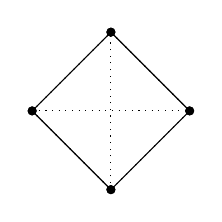
\begin{tikzpicture}[baseline=(current bounding box.center)]
  \pic at (0,0) {chamber4};
\draw (0,1) -- (1,0) -- (2,1) -- (1,2) -- (0,1);
\draw[fill] (0,1) circle [radius=0.05];
\draw[fill] (1,0) circle [radius=0.05];
\draw[fill] (2,1) circle [radius=0.05];
\draw[fill] (1,2) circle [radius=0.05];
\end{tikzpicture}
 &
$\begin{bmatrix}
1 & 0 & 1 \\
0 & 2 & 0 \\
0 & 1 & 0 \end{bmatrix}$
& $x@m = j$
\\ \hline
\begin{tikzpicture}[baseline=(current bounding box.center)]
  \pic at (0,0) {chamber1};
\draw (0.85,0) -- (0.85,1.5);
\draw[fill] (0.85, 1.5) circle [radius=0.05];
\end{tikzpicture} &
ABC, BAC &
$d$
 &
$\begin{bmatrix}
0 & 0 & 1 \\
0 & 1 & 0 \\
1 & 0 & 0 \end{bmatrix}$
& $\$x@m = d$
\\
$\begin{bmatrix}
0 & 0 & 1 & 0 & 0 \\
0 & 0 & 0 & 1/3 & 0 \\
1 & 1 & 0 & -2/3 & 1 \end{bmatrix}$ &
CAB, CBA &
$S$
 &
$\begin{bmatrix}
1 & 0 & 0 \\
0 & 1 & 0 \\
0 & 0 & 1 \end{bmatrix}$
& $\$x@m = S$
\\ &
ACB, BCA &
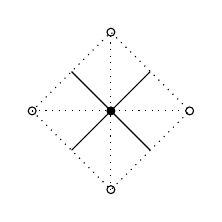
\begin{tikzpicture}[baseline=(current bounding box.center)]
  \pic at (0,0) {chamber4};
\draw (0.5,0.5) -- (1.5,1.5);
\draw (1.5,0.5) -- (0.5,1.5);
\draw[fill] (1,1) circle [radius=0.05];
\end{tikzpicture}
 &
$\begin{bmatrix}
0 & 1 & 0 \\
0 & 2 & 0 \\
1 & 0 & 1 \end{bmatrix}$
&  $x@m = a$
\end{tabular}
\end{table}

\begin{table}
\caption{$o$-cohort of LSPs}
\begin{tabular}[t]{ c|m{1cm} c c m{2cm} }
\hline \hline
$x : \mathcal{W} \to \mathcal{P}$, $M_{x}$ & $@$ & $\$x@m : \mathcal{P}_3 \to \mathcal{P}_3$ & $M_{\$x@m}$
& Note
\\ \hline
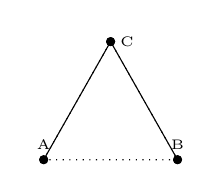
\begin{tikzpicture}[baseline=(current bounding box.center)]
  \pic at (0,0) {chamber1};
  \draw (0, 0) -- (0.85,1.5) -- (1.7, 0) ;
  \draw[fill] (0, 0) circle [radius=0.05] ;
  \draw[fill] (0.85, 1.5) circle [radius=0.05] ;
  \draw[fill] (1.7, 0) circle [radius=0.05] ;
\end{tikzpicture} &
ABC, BAC &
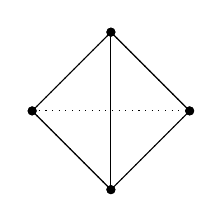
\begin{tikzpicture}[baseline=(current bounding box.center)]
  \pic at (0,0) {chamber4};
  \draw (1,0) -- (0,1) -- (1,2) -- (2,1) -- (1,0);
  \draw (1,0) -- (1,2);
  \draw[fill] (0,1) circle [radius=0.05];
  \draw[fill] (2,1) circle [radius=0.05];
  \draw[fill] (1,0) circle [radius=0.05];
  \draw[fill] (1,2) circle [radius=0.05];
\end{tikzpicture}
 &
 $\begin{bmatrix}
 1 & 0 & 1 \\
 0 & 3 & 0 \\
 0 & 2 & 0 \end{bmatrix}$
&  $\$x@m = n$
\\ $\begin{bmatrix}
1 & -2/3 & 1 \\
0 & 2/3 & 0 \\
0 & 1/3 & 0 \end{bmatrix}$ & ACB, BCA &
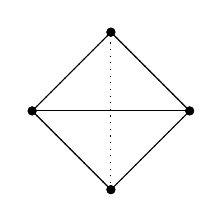
\begin{tikzpicture}[baseline=(current bounding box.center)]
  \pic at (0,0) {chamber4};
\draw (1,0) -- (0,1) -- (1,2) -- (2,1) -- (1,0);
\draw (0,1) -- (2,1);
\draw[fill] (0,1) circle [radius=0.05];
\draw[fill] (2,1) circle [radius=0.05];
\draw[fill] (1,0) circle [radius=0.05];
\draw[fill] (1,2) circle [radius=0.05];
\end{tikzpicture}
 &
 $\begin{bmatrix}
 1 & 0 & 1 \\
 0 & 3 & 0 \\
 0 & 2 & 0 \end{bmatrix}$
& $\$x@m = k$
\\ & CAB, CBA &
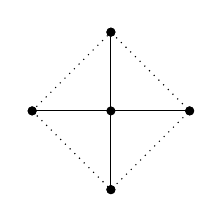
\begin{tikzpicture}[baseline=(current bounding box.center)]
  \pic at (0,0) {chamber4};
\draw (0,1) -- (2,1);
\draw (1,0) -- (1,2);
\draw[fill] (1,1) circle [radius=0.05];
\draw[fill] (0,1) circle [radius=0.05];
\draw[fill] (2,1) circle [radius=0.05];
\draw[fill] (1,0) circle [radius=0.05];
\draw[fill] (1,2) circle [radius=0.05];
\end{tikzpicture}
 &
$\begin{bmatrix}
1 & 1 & 1 \\
0 & 4 & 0 \\
0 & 2 & 0 \end{bmatrix}$
& $x@m = o$
\\ \hline
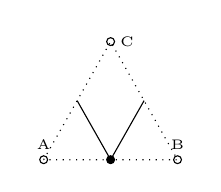
\begin{tikzpicture}[baseline=(current bounding box.center)]
  \pic at (0,0) {chamber1};
  \draw (0.425, 0.75) -- (0.85,0) -- (1.275, 0.75) ;
  \draw[fill] (0.85,0) circle [radius=0.05];
\end{tikzpicture} &
ACB, BCA &
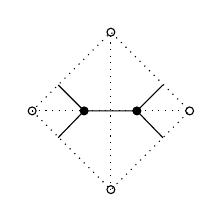
\begin{tikzpicture}[baseline=(current bounding box.center)]
  \pic at (0,0) {chamber4};
  \draw (0.33, 0.66) -- (0.66,1) -- (1.33,1) -- (1.66,1.33);
  \draw (0.33, 1.33) -- (0.66,1);
  \draw (1.33,1) -- (1.66,0.66);
  \draw[fill] (0.66,1) circle [radius=0.05];
  \draw[fill] (1.33,1) circle [radius=0.05];
\end{tikzpicture}
 &
 $\begin{bmatrix}
 0 & 2 & 0 \\
 0 & 3 & 0 \\
 1 & 0 & 1 \end{bmatrix}$
&  $\$x@m = t$
\\ $\begin{bmatrix}
0 & 1/3 & 0 \\
0 & 2/3 & 0 \\
1 & -2/3 & 1 \end{bmatrix}$ & ABC, BAC &
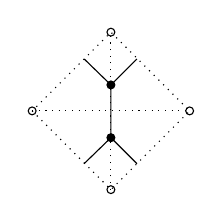
\begin{tikzpicture}[baseline=(current bounding box.center)]
  \pic at (0,0) {chamber4};
  \draw (0.66, 0.33) -- (1,0.66) -- (1,1.33) -- (1.33,1.66);
  \draw (1.33, 0.33) -- (1,0.66);
  \draw (1,1.33) -- (0.66,1.66);
  \draw[fill] (1,0.66) circle [radius=0.05];
  \draw[fill] (1,1.33) circle [radius=0.05];
\end{tikzpicture}
 &
 $\begin{bmatrix}
 0 & 2 & 0 \\
 0 & 3 & 0 \\
 1 & 0 & 1 \end{bmatrix}$
& $\$x@m = z$
\\ & CAB, CBA &
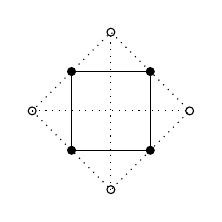
\begin{tikzpicture}[baseline=(current bounding box.center)]
  \pic at (0,0) {chamber4};
\draw (0.5,0.5) -- (1.5,0.5) -- (1.5,1.5) -- (0.5,1.5) -- (0.5,0.5);
\draw[fill] (0.5,0.5) circle [radius=0.05];
\draw[fill] (1.5,0.5) circle [radius=0.05];
\draw[fill] (1.5,1.5) circle [radius=0.05];
\draw[fill] (0.5,1.5) circle [radius=0.05];
\end{tikzpicture}
 &
$\begin{bmatrix}
0 & 2 & 0 \\
0 & 4 & 0 \\
1 & 1 & 1 \end{bmatrix}$
& $x@m = e$
\end{tabular}
\end{table}

\begin{table}[h!]
\caption{$u$-cohort of LSPs}
\begin{tabular}[t]{ c|m{1cm} c c m{2cm} }
\hline \hline
$x : \mathcal{W} \to \mathcal{P}$, $M_{x}$ & $@$ & $\$x@m : \mathcal{P}_3 \to \mathcal{P}_3$ & $M_{\$x@m}$
& Note
\\ \hline
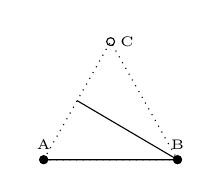
\begin{tikzpicture}[baseline=(current bounding box.center)]
  \pic at (0,0) {chamber1};
  \draw (0.425,0.75) -- (1.7, 0)  -- (0, 0);
  \draw[fill] (0, 0) circle [radius=0.05];
  \draw[fill] (1.7, 0) circle [radius=0.05];
\end{tikzpicture} &
ABC &
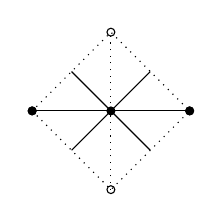
\begin{tikzpicture}[baseline=(current bounding box.center)]
  \pic at (0,0) {chamber4};
\draw (0,1) -- (2,1);
\draw (0.5,0.5) -- (1.5,1.5);
\draw (1.5,0.5) -- (0.5,1.5);
\draw[fill] (0,1) circle [radius=0.05];
\draw[fill] (1,1) circle [radius=0.05];
\draw[fill] (2,1) circle [radius=0.05];
\end{tikzpicture}
 &
$\begin{bmatrix}
1 & 1 & 0 \\
0 & 4 & 0 \\
0 & 2 & 1 \end{bmatrix}$
& $x@m = u$
\\$\begin{bmatrix}
1 & 1 & 0 & -2/3 & 1 \\
0 & 0 & 0 & 2/3 & 0 \\
0 & 0 & 1 & 1/3 & 0 \end{bmatrix}$ & ACB & $n$ &
$\begin{bmatrix}
1 & 0 & 1 \\
0 & 3 & 0 \\
0 & 2 & 0 \end{bmatrix}$
& $\$x@m = n$
\\ & BAC & $S$ &
$\begin{bmatrix}
1 & 0 & 0 \\
0 & 1 & 0 \\
0 & 0 & 1 \end{bmatrix}$
& $\$x@m = S$
\\ \hline
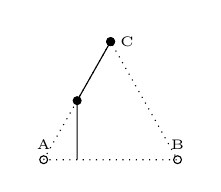
\begin{tikzpicture}[baseline=(current bounding box.center)]
  \pic at (0,0) {chamber1};
  \draw (0.85, 1.5) -- (0.425, 0.75)  -- (0.425, 0);
  \draw[fill] (0.85, 1.5) circle [radius=0.05];
  \draw[fill] (0.425, 0.75) circle [radius=0.05];
\end{tikzpicture} &
 ACB & $t$ &
$\begin{bmatrix}
0 & 2 & 0 \\
0 & 3 & 0 \\
1 & 0 & 1 \end{bmatrix}$
& $\$x@m = t$
\\$\begin{bmatrix}
0 & 0 & 1 & 1/3 & 0 \\
0 & 0 & 0 & 2/3 & 0 \\
1 & 1 & 0 & -2/3 & 1
\end{bmatrix}$ & CAB & $S$ &
$\begin{bmatrix}
1 & 0 & 0 \\
0 & 1 & 0 \\
0 & 0 & 1 \end{bmatrix}$
& $\$x@m = S$
\\ & CBA &
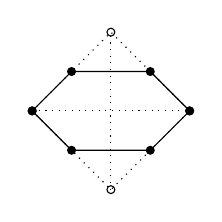
\begin{tikzpicture}[baseline=(current bounding box.center)]
  \pic at (0,0) {chamber4};
\draw (0,1) -- (0.5,0.5) -- (1.5,0.5) -- (2,1) -- (1.5,1.5) -- (0.5,1.5)
  -- (0,1);
\draw[fill] (0.5,0.5) circle [radius=0.05];
\draw[fill] (1.5,1.5) circle [radius=0.05];
\draw[fill] (1.5,0.5) circle [radius=0.05];
\draw[fill] (0.5,1.5) circle [radius=0.05];
\draw[fill] (0,1) circle [radius=0.05];
\draw[fill] (2,1) circle [radius=0.05];
\end{tikzpicture}
 &
$\begin{bmatrix}
1 & 2 & 0 \\
0 & 4 & 0 \\
0 & 1 & 1 \end{bmatrix}$
& $x@m = c$
\end{tabular}
\end{table}

\begin{table}[h!]
\caption{$l$-cohort of LSPs}
\begin{tabular}[t]{ c|m{1cm} c c m{2cm} }
\hline \hline
$x : \mathcal{W} \to \mathcal{P}$, $M_{x}$ & $@$ & $\$x@m : \mathcal{P}_3 \to \mathcal{P}_3$ & $M_{\$x@m}$
& Note
\\ \hline
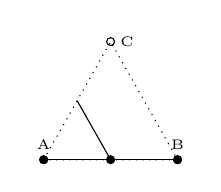
\begin{tikzpicture}[baseline=(current bounding box.center)]
  \pic at (0,0) {chamber1};
\draw[fill] (0, 0) circle [radius=0.05];
\draw[fill] (1.7, 0) circle [radius=0.05];
\draw[fill] (0.85, 0) circle [radius=0.05];
\draw (0, 0) -- (1.7, 0) ;
\draw (0.425, 0.75) -- (0.85, 0) ;
\end{tikzpicture} &
ABC&
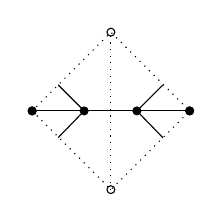
\begin{tikzpicture}[baseline=(current bounding box.center)]
  \pic at (0,0) {chamber4};
\draw (2,1) -- (0,1) ;
\draw (0.33,0.66) -- (0.66,1) -- (0.33,1.33);
\draw (1.66,0.66) -- (1.33,1) -- (1.66,1.33);
\draw[fill] (0,1) circle [radius=0.05];
\draw[fill] (0.66,1) circle [radius=0.05];
\draw[fill] (1.33,1) circle [radius=0.05];
\draw[fill] (2,1) circle [radius=0.05];
\end{tikzpicture}
 &
$\begin{bmatrix}
1 & 2 & 0 \\
0 & 5 & 0 \\
0 & 2 & 1 \end{bmatrix}$
& $\$x@m = dld$
\\ $\begin{bmatrix}
1 & 1 & 0 & -1/3 & 1 \\
0 & 0 & 0 & 1 & 0 \\
0 & 0 & 1 & 1/3 & 0 \end{bmatrix}$ & BAC& $S$ &
$\begin{bmatrix}
1 & 0 & 0 \\
0 & 1 & 0 \\
0 & 0 & 1 \end{bmatrix}$
& $\$x@m = S$
\\ & BCA&
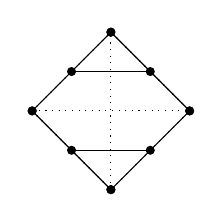
\begin{tikzpicture}[baseline=(current bounding box.center)]
  \pic at (0,0) {chamber4};
\draw (0,1) -- (1,2) -- (2,1) -- (1,0) -- (0,1);
\draw (0.5, 1.5) -- (1.5,1.5);
\draw (0.5, 0.5) -- (1.5,0.5);
\draw[fill] (0,1) circle [radius=0.05];
\draw[fill] (2,1) circle [radius=0.05];
\draw[fill] (1,0) circle [radius=0.05];
\draw[fill] (1,2) circle [radius=0.05];
\draw[fill] (0.5,0.5) circle [radius=0.05];
\draw[fill] (1.5,1.5) circle [radius=0.05];
\draw[fill] (1.5,0.5) circle [radius=0.05];
\draw[fill] (0.5,1.5) circle [radius=0.05];
\end{tikzpicture}
 &
$\begin{bmatrix}
1 & 2 & 1 \\
0 & 6 & 0 \\
0 & 3 & 0 \end{bmatrix}$
& $x@m$
\\ \hline
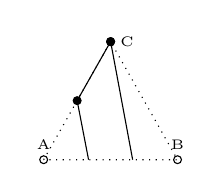
\begin{tikzpicture}[baseline=(current bounding box.center)]
  \pic at (0,0) {chamber1};
\draw[fill] (0.85, 1.5) circle [radius=0.05];
\draw[fill] (0.425, 0.75) circle [radius=0.05];
\draw (0.57, 0) -- (0.425, 0.75) -- (0.85, 1.5) -- (1.13, 0);
\end{tikzpicture} &
CBA&
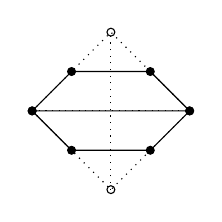
\begin{tikzpicture}[baseline=(current bounding box.center)]
  \pic at (0,0) {chamber4};
\draw (0,1) -- (2,1) -- (1.5,0.5) -- (0.5,0.5) --
      (0,1) -- (0.5,1.5) -- (1.5,1.5) -- (2,1);
\draw[fill] (0,1) circle [radius=0.05];
\draw[fill] (0.5,0.5) circle [radius=0.05];
\draw[fill] (1.5,1.5) circle [radius=0.05];
\draw[fill] (1.5,0.5) circle [radius=0.05];
\draw[fill] (0.5,1.5) circle [radius=0.05];
\draw[fill] (2,1) circle [radius=0.05];
\end{tikzpicture}
 &
$\begin{bmatrix}
1 & 2 & 0 \\
0 & 5 & 0 \\
0 & 2 & 1 \end{bmatrix}$
& $\$x@m = l$
\\ $\begin{bmatrix}
0 & 0 & 1 & 1/3 & 0 \\
0 & 0 & 0 & 1 & 0 \\
1 & 1 & 0 & -1/3 & 1 \end{bmatrix}$ & CAB& $S$ &
$\begin{bmatrix}
1 & 0 & 0 \\
0 & 1 & 0 \\
0 & 0 & 1 \end{bmatrix}$
& $\$x@m = S$
\\ & ACB&
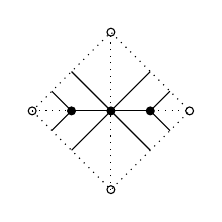
\begin{tikzpicture}[baseline=(current bounding box.center)]
  \pic at (0,0) {chamber4};
\draw (0.5, 1) -- (1.5,1);
\draw (0.5, 0.5) -- (1.5,1.5);
\draw (0.5, 1.5) -- (1.5,0.5);
\draw (0.25, 1.25) -- (0.5, 1) -- (0.25, 0.75);
\draw (1.75, 1.25) -- (1.5, 1) -- (1.75, 0.75);
\draw[fill] (0.5,1) circle [radius=0.05];
\draw[fill] (1,1) circle [radius=0.05];
\draw[fill] (1.5,1) circle [radius=0.05];
\end{tikzpicture}
 &
$\begin{bmatrix}
0 & 3 & 0 \\
0 & 6 & 0 \\
1 & 2 & 1 \end{bmatrix}$
& $x@m$
\end{tabular}
\end{table}

\begin{table}[h!]
\caption{$L_0$-cohort of LSPs}
\begin{tabular}[t]{ c|m{1cm} c c m{2cm} }
\hline \hline
$x : \mathcal{W} \to \mathcal{P}$, $M_{x}$ & $@$ & $\$x@m : \mathcal{P}_3 \to \mathcal{P}_3$ & $M_{\$x@m}$
& Note
\\ \hline
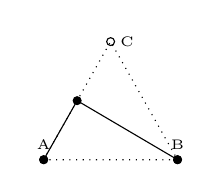
\begin{tikzpicture}[baseline=(current bounding box.center)]
  \pic at (0,0) {chamber1};
\draw[fill] (0, 0) circle [radius=0.05];
\draw[fill] (0.425, 0.75) circle [radius=0.05];
\draw[fill] (1.7, 0) circle [radius=0.05];
\draw (0,0) -- (0.425, 0.75) -- (1.7, 0);
\end{tikzpicture} &
ABC&
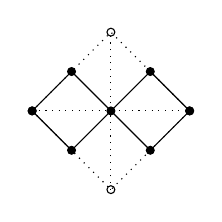
\begin{tikzpicture}[baseline=(current bounding box.center)]
  \pic at (0,0) {chamber4};
\draw (0,1) -- (0.5,0.5) -- (1.5,1.5) --
      (2,1) -- (1.5,0.5) -- (0.5,1.5) -- (0,1);
\draw[fill] (0,1) circle [radius=0.05];
\draw[fill] (1,1) circle [radius=0.05];
\draw[fill] (2,1) circle [radius=0.05];
\draw[fill] (0.5,0.5) circle [radius=0.05];
\draw[fill] (0.5,1.5) circle [radius=0.05];
\draw[fill] (1.5,1.5) circle [radius=0.05];
\draw[fill] (1.5,0.5) circle [radius=0.05];
\end{tikzpicture}
 &
$\begin{bmatrix}
1 & 3 & 0 \\
0 & 6 & 0 \\
0 & 2 & 1 \end{bmatrix}$
&${x@m = dL_0d}$
\\ $\begin{bmatrix}
1 & 1 & 0 & -1/3 & 1 \\
0 & 0 & 0 & 1 & 0 \\
0 & 0 & 1 & 1/3 & 0 \end{bmatrix}$ & BAC &
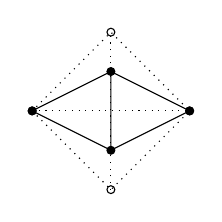
\begin{tikzpicture}[baseline=(current bounding box.center)]
  \pic at (0,0) {chamber4};
\draw (1,1.5) -- (0,1) -- (1,0.5) -- (1,1.5) -- (2,1) -- (1,0.5);
\draw[fill] (0,1) circle [radius=0.05];
\draw[fill] (1,0.5) circle [radius=0.05];
\draw[fill] (1,1.5) circle [radius=0.05];
\draw[fill] (2,1) circle [radius=0.05];
\end{tikzpicture}
 &
$\begin{bmatrix}
1 & 2 & 0 \\
0 & 5 & 0 \\
0 & 2 & 1 \end{bmatrix}$
& $\$x@m =$ Lozenge \dag
\\ & BCA &
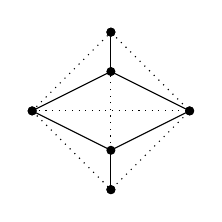
\begin{tikzpicture}[baseline=(current bounding box.center)]
  \pic at (0,0) {chamber4};
\draw (0,1) -- (1,0.5) -- (2,1) -- (1,1.5) -- (0,1);
\draw (1,0) -- (1,0.5);
\draw (1,2) -- (1,1.5);
\draw[fill] (0,1) circle [radius=0.05];
\draw[fill] (1,0) circle [radius=0.05];
\draw[fill] (1,2) circle [radius=0.05];
\draw[fill] (1,0.5) circle [radius=0.05];
\draw[fill] (1,1.5) circle [radius=0.05];
\draw[fill] (2,1) circle [radius=0.05];
\end{tikzpicture}
 &
$\begin{bmatrix}
1 & 2 & 1 \\
0 & 6 & 0 \\
0 & 3 & 0 \end{bmatrix}$
& $x@m = jk$
\\ \hline
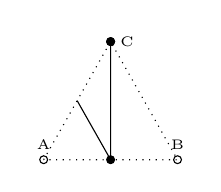
\begin{tikzpicture}[baseline=(current bounding box.center)]
  \pic at (0,0) {chamber1};
\draw (0.85,1.5) -- (0.85,0) -- (0.425, 0.75);
\draw[fill] (0.85, 1.5) circle [radius=0.05];
\draw[fill] (0.85, 0) circle [radius=0.05];
\end{tikzpicture} &
CAB &
Lozenge
 &
$\begin{bmatrix}
1 & 2 & 0 \\
0 & 5 & 0 \\
0 & 2 & 1 \end{bmatrix}$
& $\$x@m =$ Lozenge \dag
\\ $\begin{bmatrix}
0 & 0 & 1 & 1/3 & 0 \\
0 & 0 & 0 & 1 & 0 \\
1 & 1 & 0 & -1/3 & 1 \end{bmatrix}$ & CBA &
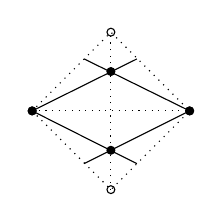
\begin{tikzpicture}[baseline=(current bounding box.center)]
  \pic at (0,0) {chamber4};
\draw (1.33,1.66) -- (0,1) -- (1.33,0.33);
\draw (0.66,1.66) -- (2,1) -- (0.66,0.33);

\draw[fill] (0,1) circle [radius=0.05];
\draw[fill] (1,0.5) circle [radius=0.05];
\draw[fill] (1,1.5) circle [radius=0.05];
\draw[fill] (2,1) circle [radius=0.05];
\end{tikzpicture}
 &
$\begin{bmatrix}
1 & 2 & 0 \\
0 & 6 & 0 \\
0 & 3 & 1 \end{bmatrix}$
& $x@m = L_0$
\\ & BCA &
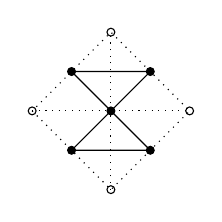
\begin{tikzpicture}[baseline=(current bounding box.center)]
  \pic at (0,0) {chamber4};
\draw (0.5,0.5) -- (1.5,0.5) --
      (0.5,1.5) -- (1.5,1.5) -- (0.5,0.5);
\draw[fill] (1,1) circle [radius=0.05];
\draw[fill] (0.5,0.5) circle [radius=0.05];
\draw[fill] (0.5,1.5) circle [radius=0.05];
\draw[fill] (1.5,1.5) circle [radius=0.05];
\draw[fill] (1.5,0.5) circle [radius=0.05];
\end{tikzpicture}
 &
$\begin{bmatrix}
0 & 3 & 0 \\
0 & 6 & 0 \\
1 & 2 & 1 \end{bmatrix}$
&$x@m = djk$
\end{tabular}
\end{table}

\begin{table}[h!]
\caption{$q$-cohort of LSPs}
\begin{tabular}[t]{ c|m{1cm} c c m{2cm} }
\hline \hline
$x : \mathcal{W} \to \mathcal{P}$, $M_{x}$ & $@$ & $\$x@m : \mathcal{P}_3 \to \mathcal{P}_3$ & $M_{\$x@m}$
& Note
\\ \hline
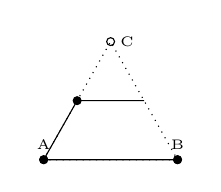
\begin{tikzpicture}[baseline=(current bounding box.center)]
  \pic at (0,0) {chamber1};
\draw[fill] (0, 0) circle [radius=0.05];
\draw[fill] (0.425, 0.75) circle [radius=0.05];
\draw[fill] (1.7, 0) circle [radius=0.05];
\draw (1.7,0) -- (0, 0) -- (0.425, 0.75) -- (1.275, 0.75) ;
\end{tikzpicture} &
ABC&
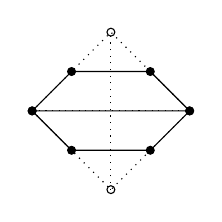
\begin{tikzpicture}[baseline=(current bounding box.center)]
  \pic at (0,0) {chamber4};
\draw (0,1) -- (2,1) -- (1.5,0.5) -- (0.5,0.5) --
      (0,1) -- (0.5,1.5) -- (1.5,1.5) -- (2,1);
\draw[fill] (0,1) circle [radius=0.05];
\draw[fill] (0.5,0.5) circle [radius=0.05];
\draw[fill] (1.5,1.5) circle [radius=0.05];
\draw[fill] (1.5,0.5) circle [radius=0.05];
\draw[fill] (0.5,1.5) circle [radius=0.05];
\draw[fill] (2,1) circle [radius=0.05];
\end{tikzpicture}
 &
$\begin{bmatrix}
1 & 2 & 0 \\
0 & 5 & 0 \\
0 & 2 & 1 \end{bmatrix}$
& $\$x@m = l$
\\ $\begin{bmatrix}
1 & 1 & 0 & -1/3 & 1 \\
0 & 0 & 0 & 1 & 0 \\
0 & 0 & 1 & 1/3 & 0 \end{bmatrix}$ & BAC &
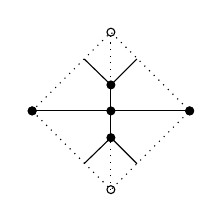
\begin{tikzpicture}[baseline=(current bounding box.center)]
  \pic at (0,0) {chamber4};
\draw (1,1.33) -- (1,0.66) ;
\draw (0,1) -- (2,1) ;
\draw (0.66,0.33) -- (1,0.66) -- (1.33,0.33);
\draw (0.66,1.66) -- (1,1.33) -- (1.33,1.66);
\draw[fill] (0,1) circle [radius=0.05];
\draw[fill] (1,1) circle [radius=0.05];
\draw[fill] (1,0.66) circle [radius=0.05];
\draw[fill] (1,1.33) circle [radius=0.05];
\draw[fill] (2,1) circle [radius=0.05];
\end{tikzpicture}
 &
$\begin{bmatrix}
1 & 3 & 0 \\
0 & 6 & 0 \\
0 & 2 & 1 \end{bmatrix}$
& $x@m = q$
\\ & ACB & $k$&
$\begin{bmatrix}
1 & 0 & 1 \\
0 & 3 & 0 \\
0 & 2 & 0 \end{bmatrix}$
& $\$x@m = k$
\\ \hline
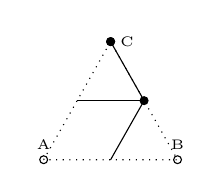
\begin{tikzpicture}[baseline=(current bounding box.center)]
  \pic at (0,0) {chamber1};
\draw (0.85,1.5) -- (1.275, 0.75) -- (0.85, 0);
\draw (1.275, 0.75) -- (0.425, 0.75);
\draw[fill] (0.85, 1.5) circle [radius=0.05];
\draw[fill] (1.275, 0.75) circle [radius=0.05];
\end{tikzpicture} &
CBA &
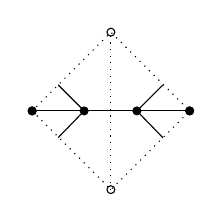
\begin{tikzpicture}[baseline=(current bounding box.center)]
  \pic at (0,0) {chamber4};
\draw (2,1) -- (0,1) ;
\draw (0.33,0.66) -- (0.66,1) -- (0.33,1.33);
\draw (1.66,0.66) -- (1.33,1) -- (1.66,1.33);
\draw[fill] (0,1) circle [radius=0.05];
\draw[fill] (0.66,1) circle [radius=0.05];
\draw[fill] (1.33,1) circle [radius=0.05];
\draw[fill] (2,1) circle [radius=0.05];
\end{tikzpicture}
 &
$\begin{bmatrix}
1 & 2 & 0 \\
0 & 5 & 0 \\
0 & 2 & 1 \end{bmatrix}$
& $\$x@m = dld$
\\ $\begin{bmatrix}
0 & 0 & 1 & 1/3 & 0 \\
0 & 0 & 0 & 1 & 0 \\
1 & 1 & 0 & -1/3 & 1 \end{bmatrix}$ & CAB &
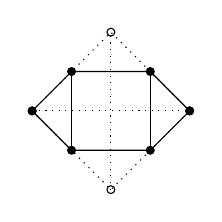
\begin{tikzpicture}[baseline=(current bounding box.center)]
  \pic at (0,0) {chamber4};
\draw (0,1) -- (0.5,0.5) -- (1.5,0.5) --
      (2,1) -- (1.5,1.5) -- (0.5,1.5) --  (0,1);
\draw (0.5,0.5) -- (0.5,1.5);
\draw (1.5,0.5) -- (1.5,1.5);
\draw[fill] (0,1) circle [radius=0.05];
\draw[fill] (0.5,0.5) circle [radius=0.05];
\draw[fill] (1.5,1.5) circle [radius=0.05];
\draw[fill] (1.5,0.5) circle [radius=0.05];
\draw[fill] (0.5,1.5) circle [radius=0.05];
\draw[fill] (2,1) circle [radius=0.05];
\end{tikzpicture}
 &
$\begin{bmatrix}
1 & 2 & 0 \\
0 & 6 & 0 \\
0 & 3 & 1 \end{bmatrix}$
& $x@m = dqd$
\\ & BCA & $t$&
$\begin{bmatrix}
0 & 2 & 0 \\
0 & 3 & 0 \\
1 & 0 & 1 \end{bmatrix}$
& $\$x@m = t$
\end{tabular}
\end{table}

\begin{table}[h!]
\caption{$m$-cohort of LSPs}
\begin{tabular}[t]{ c c|m{1cm} c c m{2cm} }
\hline \hline
$x : \mathcal{W} \to \mathcal{P}$ & $M_{x}$ & $@$ & $\$x@m : \mathcal{P}_3 \to \mathcal{P}_3$ & $M_{\$x@m}$
& Note
\\ \hline
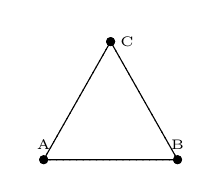
\begin{tikzpicture}[baseline=(current bounding box.center)]
  \pic at (0,0) {chamber1};
\draw (0, 0) -- (0.85,1.5) -- (1.7, 0) -- (0, 0) ;
\draw[fill] (0, 0) circle [radius=0.05];
\draw[fill] (0.85, 1.5) circle [radius=0.05];
\draw[fill] (1.7, 0) circle [radius=0.05];
\end{tikzpicture} &
$\begin{bmatrix}
1 & 0 & 0 \\
0 & 1 & 0 \\
0 & 0 & 1 \end{bmatrix}$ &
All &
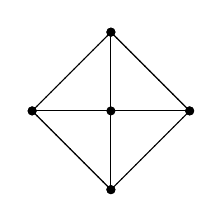
\begin{tikzpicture}[baseline=(current bounding box.center)]
  \pic at (0,0) {chamber4};
\draw (0,1) -- (1,0) -- (2,1) -- (1,2) -- (0,1);
\draw (0,1) -- (2,1);
\draw (1,0) -- (1,2);
\draw[fill] (0,1) circle [radius=0.05];
\draw[fill] (1,0) circle [radius=0.05];
\draw[fill] (1,1) circle [radius=0.05];
\draw[fill] (2,1) circle [radius=0.05];
\draw[fill] (1,2) circle [radius=0.05];
\end{tikzpicture}
 &
$\begin{bmatrix}
1 & 1 & 1 \\
0 & 6 & 0 \\
0 & 4 & 0 \end{bmatrix}$
& ${x = S}$,
${xm = m = kj}$
\\ \hline
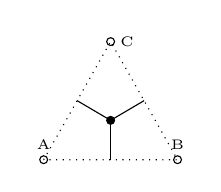
\begin{tikzpicture}[baseline=(current bounding box.center)]
  \pic at (0,0) {chamber1};
\draw (0.85, 0) -- (0.85,0.5);
\draw (0.425,0.75) -- (0.85,0.5) -- (1.275,0.75);
\draw[fill] (0.85, 0.5) circle [radius=0.05];
\end{tikzpicture} &
$\begin{bmatrix}
0 & 0 & 1 \\
0 & 1 & 0 \\
1 & 0 & 0 \end{bmatrix}$ &
All &
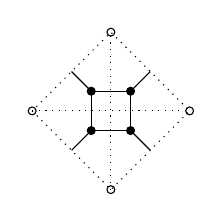
\begin{tikzpicture}[baseline=(current bounding box.center)]
  \pic at (0,0) {chamber4};
  \draw (0.75,1.25) -- (1.25,1.25) -- (1.25,0.75) -- (0.75,0.75) -- (0.75,1.25);
  \draw (0.75,1.25) -- (0.5,1.5);
  \draw (1.25,1.25) -- (1.5,1.5);
  \draw (1.25,0.75) -- (1.5,0.5);
  \draw (0.75,0.75) -- (0.5,0.5);
  \draw[fill] (0.75,1.25) circle [radius=0.05];
  \draw[fill] (1.25,1.25) circle [radius=0.05];
  \draw[fill] (1.25,0.75) circle [radius=0.05];
  \draw[fill] (0.75,0.75) circle [radius=0.05];
\end{tikzpicture}
 &
$\begin{bmatrix}
0 & 4 & 0 \\
0 & 6 & 0 \\
1 & 1 & 1 \end{bmatrix}$
& ${x = d}$,
${xm = b = ta}$
\end{tabular}
\end{table}

\begin{table}[h!]
\caption{$K$-cohort of LSPs}
\begin{tabular}[t]{ c|m{1cm} c c m{2cm} }
\hline \hline
$x : \mathcal{W} \to \mathcal{P}$, $M_{x}$ & $@$ & $\$x@m : \mathcal{P}_3 \to \mathcal{P}_3$ & $M_{\$x@m}$
& Note
\\ \hline
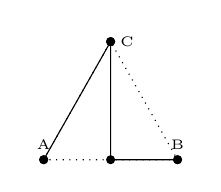
\begin{tikzpicture}[baseline=(current bounding box.center)]
  \pic at (0,0) {chamber1};
\draw[fill] (0, 0) circle [radius=0.05];
\draw[fill] (0.85, 1.5) circle [radius=0.05];
\draw[fill] (1.7, 0) circle [radius=0.05];
\draw[fill] (0.85, 0) circle [radius=0.05];
\draw (0, 0) -- (0.85, 1.5) -- (0.85, 0) -- (1.7, 0) ;
\end{tikzpicture} &
ABC&
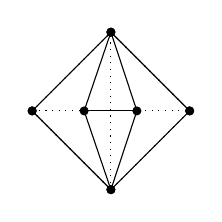
\begin{tikzpicture}[baseline=(current bounding box.center)]
  \pic at (0,0) {chamber4};
  \draw (0,1) -- (1,0) -- (2,1) -- (1,2) -- (0,1);
  \draw (0.66,1) -- (1,0) -- (1.33,1) -- (1,2) -- (0.66,1);
  \draw (0.66,1) -- (1.33,1);
  \draw[fill] (0,1) circle [radius=0.05];
  \draw[fill] (1,0) circle [radius=0.05];
  \draw[fill] (2,1) circle [radius=0.05];
  \draw[fill] (1,2) circle [radius=0.05];
  \draw[fill] (0.66,1) circle [radius=0.05];
  \draw[fill] (1.33,1) circle [radius=0.05];
\end{tikzpicture}
 &
$\begin{bmatrix}
1 & 2 & 1 \\
0 & 7 & 0 \\
0 & 4 & 0 \end{bmatrix}$
& $\$x@m$ \dag
\\ $\begin{bmatrix}
1 & -1/3 & 1 \\
0 & 4/3 & 0 \\
0 & 2/3 & 0 \end{bmatrix}$ & ACB &
\begin{tikzpicture}[baseline=(current bounding box.center)]
  \pic at (0,0) {chamber4};
  \draw (0,1) -- (2,1);
  \draw (1,0) -- (0.5,0.5) -- (1.5,1.5) --
        (1,2) -- (0.5,1.5) -- (1.5,0.5) -- (1,0);
  \draw[fill] (0,1) circle [radius=0.05];
  \draw[fill] (1,0) circle [radius=0.05];
  \draw[fill] (2,1) circle [radius=0.05];
  \draw[fill] (1,2) circle [radius=0.05];
  \draw[fill] (0.5,0.5) circle [radius=0.05];
  \draw[fill] (0.5,1.5) circle [radius=0.05];
  \draw[fill] (1.5,1.5) circle [radius=0.05];
  \draw[fill] (1.5,0.5) circle [radius=0.05];
\end{tikzpicture}
 &
$\begin{bmatrix}
1 & 3 & 1 \\
0 & 8 & 0 \\
0 & 4 & 0 \end{bmatrix}$
& $x@m$
\\ & CAB &
\begin{tikzpicture}[baseline=(current bounding box.center)]
  \pic at (0,0) {chamber4};
  \draw (0,1) -- (2,1);
  \draw (0,1) -- (1,0.5) -- (2,1) -- (1,1.5) -- (0,1);
  \draw (1,0.5) -- (1,0);
  \draw (1,1.5) -- (1,2);
  \draw[fill] (0,1) circle [radius=0.05];
  \draw[fill] (1,0) circle [radius=0.05];
  \draw[fill] (2,1) circle [radius=0.05];
  \draw[fill] (1,2) circle [radius=0.05];
  \draw[fill] (1,1.5) circle [radius=0.05];
  \draw[fill] (1,0.5) circle [radius=0.05];
\end{tikzpicture}
 &
$\begin{bmatrix}
1 & 2 & 1 \\
0 & 7 & 0 \\
0 & 4 & 0 \end{bmatrix}$
& $\$x@m = K$
\\ \hline
\begin{tikzpicture}[baseline=(current bounding box.center)]
  \pic at (0,0) {chamber1};
\draw[fill] (0.425, 0) circle [radius=0.05];
\draw[fill] (1.275, 0.75) circle [radius=0.05];
\draw (0.425, 0.75) -- (0.425, 0) -- (1.275, 0.75) -- (1.275, 0) ;
\end{tikzpicture} &
ABC &
\begin{tikzpicture}[baseline=(current bounding box.center)]
  \pic at (0,0) {chamber4};
  \draw (0.5,1) -- (1,0.5) -- (1.5,1) -- (1,1.5) -- (0.5,1);
  \draw (1,0.5) -- (1,1.5);
  \draw (0.25,0.75) -- (0.5,1) -- (0.25,1.25);
  \draw (1.75,0.75) -- (1.5,1) -- (1.75,1.25);
  \draw[fill] (0.5,1) circle [radius=0.05];
  \draw[fill] (1,0.5) circle [radius=0.05];
  \draw[fill] (1.5,1) circle [radius=0.05];
  \draw[fill] (1,1.5) circle [radius=0.05];
\end{tikzpicture}
 &
$\begin{bmatrix}
1 & 2 & 1 \\
0 & 7 & 0 \\
0 & 4 & 0 \end{bmatrix}$
& $\$x@m$ \dag
\\ $\begin{bmatrix}
0 & 2/3 & 0 \\
0 & 4/3 & 0 \\
1 & -1/3 & 1 \end{bmatrix}$ & ACB&
\begin{tikzpicture}[baseline=(current bounding box.center)]
  \pic at (0,0) {chamber4};
  \draw (0.75,1.75) -- (1,1.5) -- (1.66,1.33) --
        (1.66,0.66) -- (1, 0.5) -- (0.75, 0.25);
  \draw (1.25,1.75) -- (1,1.5) -- (0.33,1.33) --
        (0.33,0.66) -- (1, 0.5) -- (1.25, 0.25);
  \draw[fill] (0.33,1.33) circle [radius=0.05];
  \draw[fill] (1.66,1.33) circle [radius=0.05];
  \draw[fill] (1.66,0.66) circle [radius=0.05];
  \draw[fill] (0.33,0.66) circle [radius=0.05];
  \draw[fill] (1,0.5) circle [radius=0.05];
  \draw[fill] (1,1.5) circle [radius=0.05];
\end{tikzpicture}
 &
$\begin{bmatrix}
0 & 4 & 0 \\
0 & 8 & 0 \\
1 & 3 & 1 \end{bmatrix}$
& $x@m$
\\ & CAB&
\begin{tikzpicture}[baseline=(current bounding box.center)]
  \pic at (0,0) {chamber4};
  \draw (1,1.25) -- (0.5,1.5) -- (1.5,1.5) -- (1,1.25);
  \draw (1,0.75) -- (0.5,0.5) -- (1.5,0.5) -- (1,0.75);
  \draw (1,0.75) -- (1,1.25);
  \draw[fill] (0.5,1.5) circle [radius=0.05];
  \draw[fill] (1.5,1.5) circle [radius=0.05];
  \draw[fill] (1.5,0.5) circle [radius=0.05];
  \draw[fill] (0.5,0.5) circle [radius=0.05];
  \draw[fill] (1,0.75) circle [radius=0.05];
  \draw[fill] (1,1.25) circle [radius=0.05];
\end{tikzpicture}
&
$\begin{bmatrix}
0 & 4 & 0 \\
0 & 7 & 0 \\
1 & 2 & 1 \end{bmatrix}$
& $\$x@m = dK$
\end{tabular}
\end{table}

\begin{table}[h!]
\caption{$M$-cohort of LSPs}
\begin{tabular}[t]{ c|m{1cm} c c m{2cm} }
\hline \hline
$x : \mathcal{W} \to \mathcal{P}$, $M_{x}$ & $@$ & $\$x@m : \mathcal{P}_3 \to \mathcal{P}_3$ & $M_{\$x@m}$
& Note
\\ \hline
\begin{tikzpicture}[baseline=(current bounding box.center)]
  \pic at (0,0) {chamber1};
\draw[fill] (0, 0) circle [radius=0.05];
\draw[fill] (1.275, 0.75) circle [radius=0.05];
\draw[fill] (1.7, 0) circle [radius=0.05];
\draw (0, 0) -- (1.275, 0.75) -- (1.7, 0) ;
\draw (1.275, 0.75) -- (0.425, 0.75) ;
\end{tikzpicture} &
ABC&
\begin{tikzpicture}[baseline=(current bounding box.center)]
  \pic at (0,0) {chamber4};
\draw (1.33,1.66) -- (0,1) -- (1.33,0.33);
\draw (0.66,1.66) -- (2,1) -- (0.66,0.33);
\draw (1,0.5) -- (1,1.5);
\draw[fill] (0,1) circle [radius=0.05];
\draw[fill] (1,0.5) circle [radius=0.05];
\draw[fill] (1,1.5) circle [radius=0.05];
\draw[fill] (2,1) circle [radius=0.05];
\end{tikzpicture}
 &
$\begin{bmatrix}
1 & 2 & 0 \\
0 & 7 & 0 \\
0 & 4 & 1 \end{bmatrix}$
& ${\$x@m = L_{-1}}$
\\ $\begin{bmatrix}
1 & 1 & 0 & -1/3 & 1 \\
0 & 0 & 0 & 4/3 & 0 \\
0 & 0 & 1 & 2/3 & 0 \end{bmatrix}$ & BCA &
\begin{tikzpicture}[baseline=(current bounding box.center)]
  \pic at (0,0) {chamber4};
\draw (0,1) -- (2,1);
\draw (1,0) -- (0.66,1) -- (1,2) -- (1.33,1) -- (1,0);
\draw[fill] (0,1) circle [radius=0.05];
\draw[fill] (0.66,1) circle [radius=0.05];
\draw[fill] (1.33,1) circle [radius=0.05];
\draw[fill] (2,1) circle [radius=0.05];
\draw[fill] (1,0) circle [radius=0.05];
\draw[fill] (1,2) circle [radius=0.05];
\end{tikzpicture}
 &
$\begin{bmatrix}
1 & 2 & 1 \\
0 & 7 & 0 \\
0 & 4 & 0 \end{bmatrix}$
& $\$x@m = M$
\\ & BAC &
\begin{tikzpicture}[baseline=(current bounding box.center)]
  \pic at (0,0) {chamber4};
\draw (0.5,0.5) -- (1.5,1.5);
\draw (0.5,1.5) -- (1.5,0.5);
\draw (0,1) -- (0.5,0.5) -- (1.5,0.5) --
      (2,1) -- (1.5,1.5) -- (0.5,1.5) -- (0,1);
\draw[fill] (0,1) circle [radius=0.05];
\draw[fill] (1,1) circle [radius=0.05];
\draw[fill] (2,1) circle [radius=0.05];
\draw[fill] (1.5,1.5) circle [radius=0.05];
\draw[fill] (1.5,0.5) circle [radius=0.05];
\draw[fill] (0.5,0.5) circle [radius=0.05];
\draw[fill] (0.5,1.5) circle [radius=0.05];
\end{tikzpicture}
 &
$\begin{bmatrix}
1 & 3 & 0 \\
0 & 8 & 0 \\
0 & 4 & 1 \end{bmatrix}$
& $x@m$
\\ \hline
\begin{tikzpicture}[baseline=(current bounding box.center)]
  \pic at (0,0) {chamber1};
\draw[fill] (0.85, 1.5) circle [radius=0.05];
\draw[fill] (0.425, 0.75) circle [radius=0.05];
\draw[fill] (0.85, 0) circle [radius=0.05];
\draw (0.85, 1.5) -- (0.425, 0.75) -- (0.85, 0) -- (1.275, 0.75);
\end{tikzpicture} &
BCA &
\begin{tikzpicture}[baseline=(current bounding box.center)]
  \pic at (0,0) {chamber4};
\draw (1,1.33) -- (1.5,1.5) -- (1.5,0.5) -- (1,0.66) --
      (1,1.33) -- (0.5,1.5) -- (0.5,0.5) -- (1,0.66);
\draw[fill] (1.5,1.5) circle [radius=0.05];
\draw[fill] (1.5,0.5) circle [radius=0.05];
\draw[fill] (0.5,0.5) circle [radius=0.05];
\draw[fill] (0.5,1.5) circle [radius=0.05];
\draw[fill] (1,1.33) circle [radius=0.05];
\draw[fill] (1,0.66) circle [radius=0.05];
\end{tikzpicture}
 &
$\begin{bmatrix}
0 & 4 & 0 \\
0 & 7 & 0 \\
1 & 2 & 1 \end{bmatrix}$
& $\$x@m = dM$
\\ $\begin{bmatrix}
0 & 0 & 1 & 2/3 & 0 \\
0 & 0 & 0 & 4/3 & 0 \\
1 & 1 & 0 & -1/3 & 1 \end{bmatrix}$ & CBA&
\begin{tikzpicture}[baseline=(current bounding box.center)]
  \pic at (0,0) {chamber4};
\draw (1,1.33) -- (1.5,1.5) -- (2,1) -- (1.5,0.5) -- (1,0.66) --
      (1,1.33) -- (0.5,1.5) -- (0,1) -- (0.5,0.5) -- (1,0.66);
\draw[fill] (0,1) circle [radius=0.05];
\draw[fill] (1,1.33) circle [radius=0.05];
\draw[fill] (1,0.66) circle [radius=0.05];
\draw[fill] (2,1) circle [radius=0.05];
\draw[fill] (1.5,1.5) circle [radius=0.05];
\draw[fill] (1.5,0.5) circle [radius=0.05];
\draw[fill] (0.5,0.5) circle [radius=0.05];
\draw[fill] (0.5,1.5) circle [radius=0.05];
\end{tikzpicture}
 &
$\begin{bmatrix}
1 & 4 & 0 \\
0 & 7 & 0 \\
0 & 2 & 1 \end{bmatrix}$
& ${\$x@m = dL_{-1}d}$
\\ & CAB &
\begin{tikzpicture}[baseline=(current bounding box.center)]
  \pic at (0,0) {chamber4};
\draw (0,1) -- (0.66,1);
\draw (2,1) -- (1.33,1);
\draw (0.66,0.33) -- (1.33,1) -- (0.66,1.66);
\draw (1.33,0.33) -- (0.66,1) -- (1.33,1.66);
\draw[fill] (0,1) circle [radius=0.05];
\draw[fill] (0.66,1) circle [radius=0.05];
\draw[fill] (1.33,1) circle [radius=0.05];
\draw[fill] (2,1) circle [radius=0.05];
\draw[fill] (1,0.66) circle [radius=0.05];
\draw[fill] (1,1.33) circle [radius=0.05];
\end{tikzpicture}
 &
$\begin{bmatrix}
1 & 4 & 0 \\
0 & 8 & 0 \\
0 & 3 & 1 \end{bmatrix}$
& $x@m = $
\end{tabular}
\end{table}

\begin{table}[h!]
\caption{$E$-cohort of LSPs}
\begin{tabular}[t]{ c|m{1cm} c c m{2cm} }
\hline \hline
$x : \mathcal{W} \to \mathcal{P}$, $M_{x}$ & $@$ & $\$x@m : \mathcal{P}_3 \to \mathcal{P}_3$ & $M_{\$x@m}$
& Note
\\ \hline
\begin{tikzpicture}[baseline=(current bounding box.center)]
  \pic at (0,0) {chamber1};
\draw[fill] (0, 0) circle [radius=0.05];
\draw[fill] (0.425, 0.75) circle [radius=0.05];
\draw[fill] (1.7, 0) circle [radius=0.05];
\draw (0, 0) -- (1.7, 0) -- (0.425, 0.75) -- (1.275, 0.75);
\end{tikzpicture} &
ABC&
\begin{tikzpicture}[baseline=(current bounding box.center)]
  \pic at (0,0) {chamber4};
\draw (0,1) -- (2,1);
\draw (0.5,1.5) -- (1.5,1.5) -- (0.5,0.5) -- (1.5,0.5) -- (0.5,1.5);
\draw[fill] (0,1) circle [radius=0.05];
\draw[fill] (1,1) circle [radius=0.05];
\draw[fill] (0.5,0.5) circle [radius=0.05];
\draw[fill] (1.5,1.5) circle [radius=0.05];
\draw[fill] (1.5,0.5) circle [radius=0.05];
\draw[fill] (0.5,1.5) circle [radius=0.05];
\draw[fill] (2,1) circle [radius=0.05];
\end{tikzpicture}
& $\begin{bmatrix}
1 & 3 & 0 \\
0 & 8 & 0 \\
0 & 4 & 1 \end{bmatrix}$
& ${x@m = dEd}$
\\ $\begin{bmatrix}
1 & 1 & 0 & -1/3 & 1 \\
0 & 0 & 0 & 4/3 & 0 \\
0 & 0 & 1 & 2/3 & 0 \end{bmatrix}$ & ACB &
 \begin{tikzpicture}[baseline=(current bounding box.center)]
  \pic at (0,0) {chamber4};
  \draw (0,1) -- (1,0) -- (2,1) -- (1,2) -- (0,1);
  \draw (0.66,1) -- (1,0) -- (1.33,1) -- (1,2) -- (0.66,1);
  \draw (0.66,1) -- (1.33,1);
  \draw[fill] (0,1) circle [radius=0.05];
  \draw[fill] (1,0) circle [radius=0.05];
  \draw[fill] (2,1) circle [radius=0.05];
  \draw[fill] (1,2) circle [radius=0.05];
  \draw[fill] (0.66,1) circle [radius=0.05];
  \draw[fill] (1.33,1) circle [radius=0.05];
\end{tikzpicture}
& $\begin{bmatrix}
1 & 2 & 1 \\
0 & 7 & 0 \\
0 & 4 & 0 \end{bmatrix}$
& $\$x@m$ \dag
\\ & BAC &
\begin{tikzpicture}[baseline=(current bounding box.center)]
  \pic at (0,0) {chamber4};
\draw (1.33,1.66) -- (0,1) -- (1.33,0.33);
\draw (0.66,1.66) -- (2,1) -- (0.66,0.33);
\draw (0,1) -- (2,1);
\draw[fill] (0,1) circle [radius=0.05];
\draw[fill] (1,0.5) circle [radius=0.05];
\draw[fill] (1,1.5) circle [radius=0.05];
\draw[fill] (2,1) circle [radius=0.05];
\end{tikzpicture}
& $\begin{bmatrix}
1 & 2 & 0 \\
0 & 7 & 0 \\
0 & 3 & 1 \end{bmatrix}$
& $\$x@m = L$
\\ \hline
\begin{tikzpicture}[baseline=(current bounding box.center)]
  \pic at (0,0) {chamber1};
\draw[fill] (0.425, 0.75) circle [radius=0.05];
\draw[fill] (1.275, 0.75) circle [radius=0.05];
\draw[fill] (0.85, 1.5) circle [radius=0.05];
\draw (0.85, 1.5) -- (1.275, 0.75) -- (0.425, 0.75) -- (0.85,0);
\end{tikzpicture} & ACB &
 \begin{tikzpicture}[baseline=(current bounding box.center)]
   \pic at (0,0) {chamber4};
   \draw (0.5,1) -- (1,0.5) -- (1.5,1) -- (1,1.5) -- (0.5,1);
   \draw (1,0.5) -- (1,1.5);
   \draw (0.25,0.75) -- (0.5,1) -- (0.25,1.25);
   \draw (1.75,0.75) -- (1.5,1) -- (1.75,1.25);
   \draw[fill] (0.5,1) circle [radius=0.05];
   \draw[fill] (1,0.5) circle [radius=0.05];
   \draw[fill] (1.5,1) circle [radius=0.05];
   \draw[fill] (1,1.5) circle [radius=0.05];
 \end{tikzpicture}
  &
 $\begin{bmatrix}
 1 & 2 & 1 \\
 0 & 7 & 0 \\
 0 & 4 & 0 \end{bmatrix}$
 & $\$x@m$ \dag
\\ $\begin{bmatrix}
0 & 0 & 1 & 2/3 & 0 \\
0 & 0 & 0 & 4/3 & 0 \\
1 & 1 & 0 & -1/3 & 1 \end{bmatrix}$ & CAB &
\begin{tikzpicture}[baseline=(current bounding box.center)]
  \pic at (0,0) {chamber4};
\draw (0.66,1) -- (1.33,1);
\draw (0,1) -- (0.33,0.66) -- (0.66,1) -- (0.33,1.33) -- (0,1);
\draw (2,1) -- (1.66,0.66) -- (1.33,1) -- (1.66,1.33) -- (2,1);
\draw[fill] (0,1) circle [radius=0.05];
\draw[fill] (0.66,1) circle [radius=0.05];
\draw[fill] (1.33,1) circle [radius=0.05];
\draw[fill] (2,1) circle [radius=0.05];
\draw[fill] (0.33,0.66) circle [radius=0.05];
\draw[fill] (1.66,1.33) circle [radius=0.05];
\draw[fill] (1.66,0.66) circle [radius=0.05];
\draw[fill] (0.33,1.33) circle [radius=0.05];
\end{tikzpicture}
 &
$\begin{bmatrix}
1 & 4 & 0 \\
0 & 7 & 0 \\
0 & 2 & 1 \end{bmatrix}$
& ${\$x@m = dLd}$
\\ & CBA&
\begin{tikzpicture}[baseline=(current bounding box.center)]
  \pic at (0,0) {chamber4};
\draw (0,1) -- (0.33,1);
\draw (2,1) -- (1.66,1);
\draw (0.33,1) -- (0.66,0.33) -- (1.33,0.33) --
      (1.66,1) -- (1.33,1.66) -- (0.66,1.66) -- (0.33,1);
\draw[fill] (0,1) circle [radius=0.05];
\draw[fill] (0.33,1) circle [radius=0.05];
\draw[fill] (1.66,1) circle [radius=0.05];
\draw[fill] (2,1) circle [radius=0.05];
\draw[fill] (0.66,0.33) circle [radius=0.05];
\draw[fill] (1.33,1.66) circle [radius=0.05];
\draw[fill] (1.33,0.33) circle [radius=0.05];
\draw[fill] (0.66,1.66) circle [radius=0.05];
\end{tikzpicture}
 &
$\begin{bmatrix}
1 & 4 & 0 \\
0 & 8 & 0 \\
0 & 3 & 1 \end{bmatrix}$
& $x@m = E$
\end{tabular}
\end{table}

\begin{table}[h!]
\caption{$J$-cohort of LSPs}
\begin{tabular}[t]{ c|m{1cm} c c m{2cm} }
\hline \hline
$x : \mathcal{W} \to \mathcal{P}$, $M_{x}$ & $@$ & $\$x@m : \mathcal{P}_3 \to \mathcal{P}_3$ & $M_{\$x@m}$
& Note
\\ \hline
\begin{tikzpicture}[baseline=(current bounding box.center)]
  \pic at (0,0) {chamber1};
\draw[fill] (0, 0) circle [radius=0.05];
\draw[fill] (0.425, 0.75) circle [radius=0.05];
\draw[fill] (1.7, 0) circle [radius=0.05];
\draw (1.7,0) -- (0, 0) -- (0.425, 0.75) -- (1.7, 0) ;
\end{tikzpicture} &
ABC&
\begin{tikzpicture}[baseline=(current bounding box.center)]
  \pic at (0,0) {chamber4};
\draw (0,1) -- (2,1) -- (1.5,0.5) -- (0.5,1.5) --
      (0,1) -- (0.5,0.5) -- (1.5,1.5) -- (2,1);
\draw[fill] (0,1) circle [radius=0.05];
\draw[fill] (1,1) circle [radius=0.05];
\draw[fill] (0.5,0.5) circle [radius=0.05];
\draw[fill] (1.5,1.5) circle [radius=0.05];
\draw[fill] (1.5,0.5) circle [radius=0.05];
\draw[fill] (0.5,1.5) circle [radius=0.05];
\draw[fill] (2,1) circle [radius=0.05];
\end{tikzpicture}
 &
$\begin{bmatrix}
1 & 3 & 0 \\
0 & 8 & 0 \\
0 & 4 & 1 \end{bmatrix}$
& $x@m$
\\ $\begin{bmatrix}
1 & 1 & 0 & -1/3 & 1 \\
0 & 0 & 0 & 4/3 & 0 \\
0 & 0 & 1 & 2/3 & 0 \end{bmatrix}$ & BAC &
\begin{tikzpicture}[baseline=(current bounding box.center)]
  \pic at (0,0) {chamber4};
\draw (1,1.5) -- (0,1) -- (1,0.5) -- (1,1.5) -- (2,1) -- (1,0.5);
\draw (0,1) -- (2,1);
\draw[fill] (0,1) circle [radius=0.05];
\draw[fill] (1,1) circle [radius=0.05];
\draw[fill] (1,0.5) circle [radius=0.05];
\draw[fill] (1,1.5) circle [radius=0.05];
\draw[fill] (2,1) circle [radius=0.05];
\end{tikzpicture}
 &
$\begin{bmatrix}
1 & 3 & 0 \\
0 & 8 & 0 \\
0 & 4 & 1 \end{bmatrix}$
& $x@m$ \dag
\\ & BCA &
\begin{tikzpicture}[baseline=(current bounding box.center)]
  \pic at (0,0) {chamber4};
\draw (0,1) -- (1,2) -- (2,1) -- (1,0) --
      (0,1) -- (1,1.5) -- (2,1) -- (1,0.5) -- (0,1);
\draw (1,0) -- (1,0.5);
\draw (1,2) -- (1,1.5);
\draw[fill] (1,0) circle [radius=0.05];
\draw[fill] (0,1) circle [radius=0.05];
\draw[fill] (2,1) circle [radius=0.05];
\draw[fill] (1,2) circle [radius=0.05];
\draw[fill] (1,0.5) circle [radius=0.05];
\draw[fill] (1,1.5) circle [radius=0.05];
\end{tikzpicture}
 &
$\begin{bmatrix}
1 & 2 & 1 \\
0 & 8 & 0 \\
0 & 5 & 0 \end{bmatrix}$
& $x@m = J$
\\ \hline
\begin{tikzpicture}[baseline=(current bounding box.center)]
  \pic at (0,0) {chamber1};
\draw[fill] (0.85, 0.5) circle [radius=0.05];
\draw[fill] (0.85, 1.5) circle [radius=0.05];
\draw (0.85, 1.5) -- (0.85, 0);
\draw (0.85, 0.5) -- (0.425,0.75);
\end{tikzpicture} &
CBA&
\begin{tikzpicture}[baseline=(current bounding box.center)]
  \pic at (0,0) {chamber4};
  \draw (0,1) -- (0.75,1.25) -- (1.25,1.25) --
        (2,1) -- (1.25,0.75) -- (0.75,0.75) -- (0,1);
  \draw (0.75,1.25) -- (0.5,1.5);
  \draw (1.25,1.25) -- (1.5,1.5);
  \draw (1.25,0.75) -- (1.5,0.5);
  \draw (0.75,0.75) -- (0.5,0.5);
  \draw[fill] (0,1) circle [radius=0.05];
  \draw[fill] (2,1) circle [radius=0.05];
  \draw[fill] (0.75,1.25) circle [radius=0.05];
  \draw[fill] (1.25,1.25) circle [radius=0.05];
  \draw[fill] (1.25,0.75) circle [radius=0.05];
  \draw[fill] (0.75,0.75) circle [radius=0.05];
\end{tikzpicture}
 &
$\begin{bmatrix}
1 & 4 & 0 \\
0 & 8 & 0 \\
0 & 3 & 1 \end{bmatrix}$
& $x@m$
\\ $\begin{bmatrix}
0 & 0 & 1 & 2/3 & 0 \\
0 & 0 & 0 & 4/3 & 0 \\
1 & 1 & 0 & -1/3 & 1 \end{bmatrix}$ & CAB &
\begin{tikzpicture}[baseline=(current bounding box.center)]
  \pic at (0,0) {chamber4};
  \draw (0,1) -- (0.75,1.25) -- (1.25,1.25) --
        (2,1) -- (1.25,0.75) -- (0.75,0.75) -- (0,1);
  \draw (0.75,1.25) -- (0.75,0.75);
  \draw (1.25,1.25) -- (1.25,0.75);
  \draw[fill] (0,1) circle [radius=0.05];
  \draw[fill] (2,1) circle [radius=0.05];
  \draw[fill] (0.75,1.25) circle [radius=0.05];
  \draw[fill] (1.25,1.25) circle [radius=0.05];
  \draw[fill] (1.25,0.75) circle [radius=0.05];
  \draw[fill] (0.75,0.75) circle [radius=0.05];
\end{tikzpicture}
 &
$\begin{bmatrix}
1 & 4 & 0 \\
0 & 8 & 0 \\
0 & 3 & 1 \end{bmatrix}$
& $x@m$ \dag
\\ & BCA &
\begin{tikzpicture}[baseline=(current bounding box.center)]
  \pic at (0,0) {chamber4};
\draw (0.75,0.75) -- (1.25,0.75);
\draw (0.75,1.25) -- (1.25,1.25);
\draw (0.5,0.5) -- (1.5,1.5);
\draw (0.5,1.5) -- (1.5,0.5);
\draw[fill] (1,1) circle [radius=0.05];
\draw[fill] (0.75,0.75) circle [radius=0.05];
\draw[fill] (0.75,1.25) circle [radius=0.05];
\draw[fill] (1.25,1.25) circle [radius=0.05];
\draw[fill] (1.25,0.75) circle [radius=0.05];
\end{tikzpicture}
 &
$\begin{bmatrix}
0 & 5 & 0 \\
0 & 8 & 0 \\
1 & 2 & 1 \end{bmatrix}$
& $x@m = dJ$
\end{tabular}
\end{table}

\begin{table}[h!]
\caption{$W$-cohort of LSPs}
\begin{tabular}[t]{ c|m{1cm} c c m{2cm} }
\hline \hline
$x : \mathcal{W} \to \mathcal{P}$, $M_{x}$ & $@$ & $\$x@m : \mathcal{P}_3 \to \mathcal{P}_3$ & $M_{\$x@m}$
& Note
\\ \hline
\begin{tikzpicture}[baseline=(current bounding box.center)]
  \pic at (0,0) {chamber1};
\draw[fill] (0, 0) circle [radius=0.05];
\draw[fill] (0.425, 0.75) circle [radius=0.05];
\draw[fill] (0.85, 0) circle [radius=0.05];
\draw[fill] (0.85, 1.5) circle [radius=0.05];
\draw[fill] (1.7, 0) circle [radius=0.05];
\draw (0,0) -- (0.85, 1.5);
\draw (0.425, 0.75) -- (0.85, 0) -- (1.7, 0);
\end{tikzpicture} &
ABC&
\begin{tikzpicture}[baseline=(current bounding box.center)]
  \pic at (0,0) {chamber4};
\draw (0,1) -- (1,0) -- (2,1) -- (1,2) -- (0,1);
\draw (0.5,0.5) -- (0.66,1) -- (0.5,1.5);
\draw (1.5,0.5) -- (1.33,1) -- (1.5,1.5);
\draw (0.66,1) -- (1.33,1);
\draw[fill] (0,1) circle [radius=0.05];
\draw[fill] (2,1) circle [radius=0.05];
\draw[fill] (1,0) circle [radius=0.05];
\draw[fill] (1,2) circle [radius=0.05];
\draw[fill] (0.5,0.5) circle [radius=0.05];
\draw[fill] (1.5,1.5) circle [radius=0.05];
\draw[fill] (1.5,0.5) circle [radius=0.05];
\draw[fill] (0.5,1.5) circle [radius=0.05];
\draw[fill] (1.33,1) circle [radius=0.05];
\draw[fill] (0.66,1) circle [radius=0.05];
\end{tikzpicture}
 &
$\begin{bmatrix}
1 & 4 & 1 \\
0 & 9 & 0 \\
0 & 4 & 0 \end{bmatrix}$
& $\$x@m = W$
\\ $\begin{bmatrix}
1 & 0 & 1 \\
0 & 5/3 & 0 \\
0 & 2/3 & 0 \end{bmatrix}$ & BCA &
\begin{tikzpicture}[baseline=(current bounding box.center)]
  \pic at (0,0) {chamber4};
\draw (1,2) -- (1,0);
\draw (0,1) -- (0.5,0.5) -- (1.5,0.5) --
      (2,1) -- (1.5,1.5) -- (0.5,1.5) -- (0,1);
\draw[fill] (0,1) circle [radius=0.05];
\draw[fill] (2,1) circle [radius=0.05];
\draw[fill] (1,0) circle [radius=0.05];
\draw[fill] (1,2) circle [radius=0.05];
\draw[fill] (1,1.5) circle [radius=0.05];
\draw[fill] (1,0.5) circle [radius=0.05];
\draw[fill] (1.5,1.5) circle [radius=0.05];
\draw[fill] (1.5,0.5) circle [radius=0.05];
\draw[fill] (0.5,0.5) circle [radius=0.05];
\draw[fill] (0.5,1.5) circle [radius=0.05];
\end{tikzpicture}
&
$\begin{bmatrix}
1 & 4 & 1 \\
0 & 9 & 0 \\
0 & 4 & 0 \end{bmatrix}$
& $\$x@m$
\\ & CAB &
\begin{tikzpicture}[baseline=(current bounding box.center)]
  \pic at (0,0) {chamber4};
\draw (2,1) -- (0,1);
\draw (1,1.5) -- (0.5,1) -- (1,0.5) -- (1.5,1) -- (1,1.5);
\draw (1,2) -- (1,1.5);
\draw (1,0) -- (1,0.5);
\draw[fill] (0,1) circle [radius=0.05];
\draw[fill] (2,1) circle [radius=0.05];
\draw[fill] (1,0) circle [radius=0.05];
\draw[fill] (1,2) circle [radius=0.05];
\draw[fill] (1,1.5) circle [radius=0.05];
\draw[fill] (1,0.5) circle [radius=0.05];
\draw[fill] (1.5,1) circle [radius=0.05];
\draw[fill] (0.5,1) circle [radius=0.05];
\end{tikzpicture}
&
$\begin{bmatrix}
1 & 4 & 1 \\
0 & 9 & 0 \\
0 & 4 & 0 \end{bmatrix}$
& $\$x@m$
\\ \hline
\begin{tikzpicture}[baseline=(current bounding box.center)]
  \pic at (0,0) {chamber1};
\draw[fill] (1.275, 0.75) circle [radius=0.05];
\draw[fill] (0.85, 0) circle [radius=0.05];
\draw (1.275, 0) -- (1.275, 0.75) -- (0.85, 0) -- (0.213,0.375);
\draw (1.275, 0.75) -- (0.638,1.125);
\end{tikzpicture} &
ABC&
\begin{tikzpicture}[baseline=(current bounding box.center)]
  \pic at (0,0) {chamber4};
\draw (1,0.5) -- (1,1.5);
\draw (0.25,1.25) -- (1.25,0.25);
\draw (0.25,0.75) -- (1.25,1.75);
\draw (1.75,1.25) -- (0.75,0.25);
\draw (1.75,0.75) -- (0.75,1.75);
\draw[fill] (1,1.5) circle [radius=0.05];
\draw[fill] (1,0.5) circle [radius=0.05];
\draw[fill] (1.5,1) circle [radius=0.05];
\draw[fill] (0.5,1) circle [radius=0.05];
\end{tikzpicture}
 &
$\begin{bmatrix}
0 & 4 & 0 \\
0 & 9 & 0 \\
1 & 4 & 1 \end{bmatrix}$
& $\$x@m = dW$
\\ $\begin{bmatrix}
0 & 2/3 & 0 \\
0 & 5/3 & 0 \\
1 & 0 & 1 \end{bmatrix}$ & BCA &
\begin{tikzpicture}[baseline=(current bounding box.center)]
  \pic at (0,0) {chamber4};
\draw (0.5,1) -- (1.5,1);
\draw (0.25,1.25) -- (0.5,1) -- (0.25,0.75);
\draw (1.75,1.25) -- (1.5,1) -- (1.75,0.75);
\draw (0.5,0.5) -- (1.5,0.5) --
      (1.5,1.5) -- (0.5,1.5) -- (0.5,0.5);
\draw[fill] (0.5,1) circle [radius=0.05];
\draw[fill] (1.5,1) circle [radius=0.05];
\draw[fill] (1.5,1.5) circle [radius=0.05];
\draw[fill] (1.5,0.5) circle [radius=0.05];
\draw[fill] (0.5,0.5) circle [radius=0.05];
\draw[fill] (0.5,1.5) circle [radius=0.05];
\end{tikzpicture}
&
$\begin{bmatrix}
0 & 4 & 0 \\
0 & 9 & 0 \\
1 & 4 & 1 \end{bmatrix}$
& $\$x@m$
\\ & CAB &
\begin{tikzpicture}[baseline=(current bounding box.center)]
  \pic at (0,0) {chamber4};
\draw (0.5,0.5) -- (1.5,0.5) --
      (1.5,1.5) -- (0.5,1.5) -- (0.5,0.5);
\draw (1,0.75) -- (1,1.25);
\draw (0.5,0.5) -- (1,0.75) -- (1.5,0.5);
\draw (0.5,1.5) -- (1,1.25) -- (1.5,1.5);
\draw[fill] (1,0.75) circle [radius=0.05];
\draw[fill] (1,1.25) circle [radius=0.05];
\draw[fill] (1.5,1.5) circle [radius=0.05];
\draw[fill] (1.5,0.5) circle [radius=0.05];
\draw[fill] (0.5,0.5) circle [radius=0.05];
\draw[fill] (0.5,1.5) circle [radius=0.05];
\end{tikzpicture}
&
$\begin{bmatrix}
0 & 4 & 0 \\
0 & 9 & 0 \\
1 & 4 & 1 \end{bmatrix}$
& $\$x@m$
\end{tabular}
\end{table}

\begin{table}[h!]
\caption{$M_n$-cohort of LSPs, $n=2k, k \ge 1$}
\begin{tabular}[t]{ c|m{1cm} c c m{2cm} }
\hline \hline
$x : \mathcal{W} \to \mathcal{P}$, $M_{x}$ & $@$ & $\$x@m : \mathcal{P}_3 \to \mathcal{P}_3$ & $M_{\$x@m}$
& Note
\\ \hline
\begin{tikzpicture}[baseline=(current bounding box.center)]
  \pic at (0,0) {chamber1};
\draw[fill] (0, 0) circle [radius=0.05];
\draw[fill] (0.85, 0) node[anchor=center] {\tiny x} node[anchor=north] {\tiny $k$};
\draw[fill] (1.7, 0) circle [radius=0.05];
\draw[fill] (0.85, 1.5) circle [radius=0.05];
\draw (0,0) -- (1.7, 0);
\draw[dashed] (0.85, 0) -- (0.85, 1.5);
\end{tikzpicture} &
ABC BAC&
\begin{tikzpicture}[baseline=(current bounding box.center)]
  \pic at (0,0) {chamber4};
\draw[fill] (0,1) circle [radius=0.05];
\draw[fill] (2,1) circle [radius=0.05];
\draw[fill] (1,0) circle [radius=0.05];
\draw[fill] (1,2) circle [radius=0.05];
\draw[fill] (0.5,1) node[anchor=center] {\tiny x} ;
\draw[fill] (1.5,1) node[anchor=center] {\tiny x} ;
\draw (0,1) -- (2,1);
\draw[dashed] (1,2) -- (0.5,1) -- (1,0) -- (1.5,1) -- (1,2);
\end{tikzpicture}
 &
 $\begin{bmatrix}
 1 & n & 1 \\
 0 & 3n+1 & 0 \\
 0 & 2n & 0 \end{bmatrix}$
& $\$x@m = M_n$
\\ $\begin{bmatrix}
1 & \frac{k-2}{3} & 1 \\
0 & k+\frac{1}{3} & 0 \\
0 & \frac{2}{3}k & 0 \end{bmatrix}$ & BCA ACB&
\begin{tikzpicture}[baseline=(current bounding box.center)]
  \pic at (0,0) {chamber4};
\draw[fill] (0,1) circle [radius=0.05];
\draw[fill] (2,1) circle [radius=0.05];
\draw[fill] (1,0) circle [radius=0.05];
\draw[fill] (1,2) circle [radius=0.05];
\draw[fill] (1,1) circle [radius=0.05];
\draw[fill] (0.5,0.5) node[anchor=center] {\tiny x} ;
\draw[fill] (1.5,0.5) node[anchor=center] {\tiny x} ;
\draw[fill] (0.5,1.5) node[anchor=center] {\tiny x} ;
\draw[fill] (1.5,1.5) node[anchor=center] {\tiny x} ;
\draw (0,1) -- (1,0) -- (2,1) -- (1,2) -- (0,1);
\draw[dashed] (0.5,0.5) -- (1.5,1.5);
\draw[dashed] (0.5,1.5) -- (1.5,0.5);
\end{tikzpicture}
 &
 $\begin{bmatrix}
 1 & n+1 & 1 \\
 0 & 3n+2 & 0 \\
 0 & 2n & 0 \end{bmatrix}$
& $x@m$
\\ \hline
\begin{tikzpicture}[baseline=(current bounding box.center)]
  \pic at (0,0) {chamber1};
\draw[fill] (0.85, 0) node[anchor=north] {\tiny $k$};
\draw[fill] (0.425, 0.75) node[anchor=center] {\tiny x} ;
\draw[fill] (1.275, 0.75) node[anchor=center] {\tiny x} ;
\draw[dashed] (0.425, 0) -- (0.425, 0.75);
\draw[dashed] (1.275, 0) -- (1.275, 0.75);
\draw (0.425,0.75) -- (1.275,0.75);
\end{tikzpicture} &
ABC BAC&
\begin{tikzpicture}[baseline=(current bounding box.center)]
  \pic at (0,0) {chamber4};
\draw[fill] (0.5,0.5) node[anchor=center] {\tiny x} ;
\draw[fill] (1,0.5) node[anchor=center] {\tiny x} ;
\draw[fill] (1.5,0.5) node[anchor=center] {\tiny x} ;
\draw[fill] (0.5,1.5) node[anchor=center] {\tiny x} ;
\draw[fill] (1,1.5) node[anchor=center] {\tiny x} ;
\draw[fill] (1.5,1.5) node[anchor=center] {\tiny x} ;
\draw (0.5,0.5) -- (1.5,0.5);
\draw (0.5,1.5) -- (1.5,1.5);
\draw[dashed] (0.5,0.5) -- (0.5,1.5);
\draw[dashed] (1,0.5) -- (1,1.5);
\draw[dashed] (1.5,0.5) -- (1.5,1.5);
\end{tikzpicture}
 &
 $\begin{bmatrix}
 0 & 2n & 0 \\
 0 & 3n+1 & 0 \\
 1 & n & 1 \end{bmatrix}$
& $\$x@m$
\\ $\begin{bmatrix}
0 & \frac{2}{3}k & 0 \\
0 & k+\frac{1}{3} & 0 \\
1 & \frac{k-2}{3} & 1 \end{bmatrix}$ & BCA ACB&
\begin{tikzpicture}[baseline=(current bounding box.center)]
  \pic at (0,0) {chamber4};
\draw[fill] (0.7,1) node[anchor=center] {\tiny x} ;
\draw[fill] (1,0.7) node[anchor=center] {\tiny x} ;
\draw[fill] (1.3,1) node[anchor=center] {\tiny x} ;
\draw[fill] (1,1.3) node[anchor=center] {\tiny x} ;
\draw (0.7,1) -- (1,0.7) -- (1.3,1) -- (1,1.3) -- (0.7,1);
\draw[dashed] (0.7,1) -- (0.35,0.65);
\draw[dashed] (1,0.7) -- (0.65,0.35);
\draw[dashed] (1,0.7) -- (1.35,0.35);
\draw[dashed] (1.3,1) -- (1.65,0.65);
\draw[dashed] (1.3,1) -- (1.65,1.35);
\draw[dashed] (1,1.3) -- (1.35,1.65);
\draw[dashed] (1,1.3) -- (0.65,1.65);
\draw[dashed] (0.7,1) -- (0.35,1.35);
\end{tikzpicture}
 &
 $\begin{bmatrix}
 0 & 2n & 0 \\
 0 & 3n + 2 & 0 \\
 1 & n + 1 & 1 \end{bmatrix}$
& $x@m$
\end{tabular}
\end{table}

\begin{table}[h!]
\caption{$M_n$/$m_n$-cohort of LSPs}
\begin{tabular}[t]{ c|m{1cm} c c m{2cm} }
\hline \hline
$x : \mathcal{W} \to \mathcal{P}$, $M_{x}$ & $@$ & $\$x@m : \mathcal{P}_3 \to \mathcal{P}_3$ & $M_{\$x@m}$
& Note
\\ \hline
\begin{tikzpicture}[baseline=(current bounding box.center)]
  \pic at (0,0) {chamber1};
\draw[fill] (0, 0) circle [radius=0.05];
\draw[fill] (0.85, 0) node[anchor=center] {\tiny x} node[anchor=north] {\tiny $k$};
\draw[fill] (1.7, 0) circle [radius=0.05];
\draw[fill] (0.85, 1.5) circle [radius=0.05];
\draw (0.85, 1.5) -- (0,0) -- (1.7, 0);
\draw[dashed] (0.85, 0) -- (0.85, 1.5);
\end{tikzpicture} &
ABC&
\begin{tikzpicture}[baseline=(current bounding box.center)]
  \pic at (0,0) {chamber4};
\draw[fill] (0,1) circle [radius=0.05];
\draw[fill] (2,1) circle [radius=0.05];
\draw[fill] (1,0) circle [radius=0.05];
\draw[fill] (1,2) circle [radius=0.05];
\draw[fill] (0.5,1) node[anchor=center] {\tiny x} ;
\draw[fill] (1.5,1) node[anchor=center] {\tiny x} ;
\draw (0,1) -- (2,1);
\draw (0,1) -- (1,0) -- (2,1) -- (1,2) -- (0,1);
\draw[dashed] (1,2) -- (0.5,1) -- (1,0) -- (1.5,1) -- (1,2);
\end{tikzpicture}
 &
$\begin{bmatrix}
1 & n & 1 \\
0 & 3n+3 & 0 \\
0 & 2n+2 & 0 \end{bmatrix}$
& ${n=2k}$, ${k \ge 0}$, ${\$x@m = m_n}$
\\ $\begin{bmatrix}
1 & \frac{2k-5}{6} & 1 \\
0 & k + \frac{1}{6} & 0 \\
0 & \frac{2}{3}k & 0 \end{bmatrix}$ & BAC&
\begin{tikzpicture}[baseline=(current bounding box.center)]
  \pic at (0,0) {chamber4};
\draw[fill] (0,1) circle [radius=0.05];
\draw[fill] (2,1) circle [radius=0.05];
\draw[fill] (1,0) circle [radius=0.05];
\draw[fill] (1,2) circle [radius=0.05];
\draw[fill] (1,1) circle [radius=0.05];
\draw[fill] (0.5,1) node[anchor=center] {\tiny x} ;
\draw[fill] (1.5,1) node[anchor=center] {\tiny x} ;
\draw (0,1) -- (2,1);
\draw (1,0) -- (1,2);
\draw[dashed] (1,2) -- (0.5,1) -- (1,0) -- (1.5,1) -- (1,2);
\end{tikzpicture}
 &
$\begin{bmatrix}
1 & n & 1 \\
0 & 3n+1 & 0 \\
0 & 2n & 0 \end{bmatrix}$
& ${n=2k+1}$, ${k \ge 0}$, ${x@m = M_n}$
\\ & ACB&
\begin{tikzpicture}[baseline=(current bounding box.center)]
  \pic at (0,0) {chamber4};
\draw[fill] (0,1) circle [radius=0.05];
\draw[fill] (2,1) circle [radius=0.05];
\draw[fill] (1,0) circle [radius=0.05];
\draw[fill] (1,2) circle [radius=0.05];
\draw[fill] (1,1) circle [radius=0.05];
\draw[fill] (0.5,0.5) node[anchor=center] {\tiny x} ;
\draw[fill] (1.5,0.5) node[anchor=center] {\tiny x} ;
\draw[fill] (0.5,1.5) node[anchor=center] {\tiny x} ;
\draw[fill] (1.5,1.5) node[anchor=center] {\tiny x} ;
\draw (0,1) -- (2,1);
\draw (0,1) -- (1,0) -- (2,1) -- (1,2) -- (0,1);
\draw[dashed] (0.5,0.5) -- (1.5,1.5);
\draw[dashed] (0.5,1.5) -- (1.5,0.5);
\end{tikzpicture}
 &
 $\begin{bmatrix}
 1 & n & 1 \\
 0 & 3n+1 & 0 \\
 0 & 2n & 0 \end{bmatrix}$
& ${n=2k}$, ${k \ge 1}$, ${x@m}$
\\ \hline
\begin{tikzpicture}[baseline=(current bounding box.center)]
  \pic at (0,0) {chamber1};
\draw[fill] (0.85, 0) node[anchor=north] {\tiny $k$};
\draw[fill] (0.708, 0.75) node[anchor=center] {\tiny x} ;
\draw[fill] (1.275, 0.75) node[anchor=center] {\tiny x} ;
\draw[dashed] (0.708, 0) -- (0.708, 0.75);
\draw[dashed] (1.275, 0) -- (1.275, 0.75);
\draw (0.425,0.75) -- (1.275,0.75);
\end{tikzpicture} & ABC&
\begin{tikzpicture}[baseline=(current bounding box.center)]
  \pic at (0,0) {chamber4};
  \draw[fill] (0.75,0.5) node[anchor=center] {\tiny x} ;
  \draw[fill] (1,0.5) node[anchor=center] {\tiny x} ;
  \draw[fill] (1.25,0.5) node[anchor=center] {\tiny x} ;
  \draw[fill] (0.75,1.5) node[anchor=center] {\tiny x} ;
  \draw[fill] (1,1.5) node[anchor=center] {\tiny x} ;
  \draw[fill] (1.25,1.5) node[anchor=center] {\tiny x} ;
  \draw (0.5,0.5) -- (1.5,0.5);
  \draw (0.5,1.5) -- (1.5,1.5);
  \draw[dashed] (0.75,0.5) -- (0.75,1.5);
  \draw[dashed] (1,0.5) -- (1,1.5);
  \draw[dashed] (1.25,0.5) -- (1.25,1.5);
\end{tikzpicture}
 &
 $\begin{bmatrix}
 0 & 2n+2 & 0 \\
 0 & 3n+3 & 0 \\
 1 & n & 1 \end{bmatrix}$
& ${n=2k}$, ${k \ge 0}$, ${\$x@m = b_n}$
\\ $\begin{bmatrix}
0 & \frac{2}{3}k & 0 \\
0 & k + \frac{1}{6} & 0 \\
1 & \frac{2k-5}{6} & 1 \end{bmatrix}$& BAC&
\begin{tikzpicture}[baseline=(current bounding box.center)]
  \pic at (0,0) {chamber4};
  \draw[fill] (0.5,0.5) node[anchor=center] {\tiny x} ;
  \draw[fill] (0.83,0.5) node[anchor=center] {\tiny x} ;
  \draw[fill] (1.17,0.5) node[anchor=center] {\tiny x} ;
  \draw[fill] (1.5,0.5) node[anchor=center] {\tiny x} ;
  \draw[fill] (0.5,1.5) node[anchor=center] {\tiny x} ;
  \draw[fill] (0.83,1.5) node[anchor=center] {\tiny x} ;
  \draw[fill] (1.17,1.5) node[anchor=center] {\tiny x} ;
  \draw[fill] (1.5,1.5) node[anchor=center] {\tiny x} ;
  \draw (0.5,0.5) -- (1.5,0.5);
  \draw (0.5,1.5) -- (1.5,1.5);
  \draw[dashed] (0.5,0.5) -- (0.5,1.5);
  \draw[dashed] (0.83,0.5) -- (0.83,1.5);
  \draw[dashed] (1.17,0.5) -- (1.17,1.5);
  \draw[dashed] (1.5,0.5) -- (1.5,1.5);
\end{tikzpicture}
 &
 $\begin{bmatrix}
 0 & 2n & 0 \\
 0 & 3n+1 & 0 \\
 1 & n & 1 \end{bmatrix}$
& ${n = 2k+1}$, ${k \ge 0}$, $x@m$
\\ & ACB&
\begin{tikzpicture}[baseline=(current bounding box.center)]
  \pic at (0,0) {chamber4};
\draw[fill] (0.6,0.9) node[anchor=center] {\tiny x} ;
\draw[fill] (1,0.6) node[anchor=center] {\tiny x} ;
\draw[fill] (1.4,0.9) node[anchor=center] {\tiny x} ;
\draw[fill] (1.4,1.1) node[anchor=center] {\tiny x} ;
\draw[fill] (1,1.4) node[anchor=center] {\tiny x} ;
\draw[fill] (0.6,1.1) node[anchor=center] {\tiny x} ;
\draw (0.6,0.9) -- (1,0.6) -- (1.4,0.9) --
(1.4,1.1) -- (1,1.4)  -- (0.6,1.1) -- (0.6,0.9);
\draw[dashed] (0.6,0.9) -- (0.35,0.65);
\draw[dashed] (1,0.6) -- (0.7,0.3);
\draw[dashed] (1,0.6) -- (1.3,0.3);
\draw[dashed] (1.4,0.9) -- (1.65,0.65);
\draw[dashed] (1.4,1.1) -- (1.65,1.35);
\draw[dashed] (1,1.4) -- (1.3,1.7);
\draw[dashed] (1,1.4) -- (0.7,1.7);
\draw[dashed] (0.6,1.1) -- (0.35,1.35);
\end{tikzpicture}
 &
 $\begin{bmatrix}
 0 & 2n & 0 \\
 0 & 3n+1 & 0 \\
 1 & n & 1 \end{bmatrix}$
& ${n=2k}$, ${k \ge 1}$, $x@m$
\end{tabular}
\end{table}

\begin{table}[h!]
\caption{$m_n$-cohort of LSPs, $n=2k+1, k \ge 0$}
\begin{tabular}[t]{ c|m{1cm} c c m{2cm} }
\hline \hline
$x : \mathcal{W} \to \mathcal{P}$, $M_{x}$ & $@$ & $\$x@m : \mathcal{P}_3 \to \mathcal{P}_3$ & $M_{\$x@m}$
& Note
\\ \hline
\begin{tikzpicture}[baseline=(current bounding box.center)]
  \pic at (0,0) {chamber1};
\draw[fill] (0, 0) circle [radius=0.05];
\draw[fill] (0.85, 0) node[anchor=center] {\tiny x} node[anchor=north] {\tiny $k$};
\draw[fill] (1.7, 0) circle [radius=0.05];
\draw[fill] (0.85, 1.5) circle [radius=0.05];
\draw (0,0) -- (1.7, 0) -- (0.85, 1.5) -- (0,0);
\draw[dashed] (0.85, 0) -- (0.85, 1.5);
\end{tikzpicture} &
ABC BAC&
\begin{tikzpicture}[baseline=(current bounding box.center)]
  \pic at (0,0) {chamber4};
\draw[fill] (0,1) circle [radius=0.05];
\draw[fill] (2,1) circle [radius=0.05];
\draw[fill] (1,0) circle [radius=0.05];
\draw[fill] (1,2) circle [radius=0.05];
\draw[fill] (1,1) circle [radius=0.05];
\draw[fill] (0.5,1) node[anchor=center] {\tiny x} ;
\draw[fill] (1.5,1) node[anchor=center] {\tiny x} ;
\draw (0,1) -- (2,1);
\draw (1,0) -- (1,2);
\draw (0,1) -- (1,0) -- (2,1) -- (1,2) -- (0,1);
\draw[dashed] (1,2) -- (0.5,1) -- (1,0) -- (1.5,1) -- (1,2);
\end{tikzpicture}
 &
 $\begin{bmatrix}
 1 & n & 1 \\
 0 & 3n+3 & 0 \\
 0 & 2n+2 & 0 \end{bmatrix}$
& $x@m = m_n$
\\ $\begin{bmatrix}
1 & \frac{2k-5}{6} & 1 \\
0 & k + \frac{1}{2} & 0 \\
0 & \frac{2k+1}{3} & 0 \end{bmatrix}$ & BCA ACB&
\begin{tikzpicture}[baseline=(current bounding box.center)]
  \pic at (0,0) {chamber4};
\draw[fill] (0,1) circle [radius=0.05];
\draw[fill] (2,1) circle [radius=0.05];
\draw[fill] (1,0) circle [radius=0.05];
\draw[fill] (1,2) circle [radius=0.05];
\draw[fill] (1,1) circle [radius=0.05];
\draw[fill] (0.5,0.5) node[anchor=center] {\tiny x} ;
\draw[fill] (1.5,0.5) node[anchor=center] {\tiny x} ;
\draw[fill] (0.5,1.5) node[anchor=center] {\tiny x} ;
\draw[fill] (1.5,1.5) node[anchor=center] {\tiny x} ;
\draw (0,1) -- (2,1);
\draw (1,0) -- (1,2);
\draw (0,1) -- (1,0) -- (2,1) -- (1,2) -- (0,1);
\draw[dashed] (0.5,0.5) -- (1.5,1.5);
\draw[dashed] (0.5,1.5) -- (1.5,0.5);
\end{tikzpicture}
 &
 $\begin{bmatrix}
 1 & n & 1 \\
 0 & 3n+3 & 0 \\
 0 & 2n+2 & 0 \end{bmatrix}$
& $x@m$
\\ \hline
\begin{tikzpicture}[baseline=(current bounding box.center)]
  \pic at (0,0) {chamber1};
\draw[fill] (0.85, 0) node[anchor=north] {\tiny $k$};
\draw[fill] (0.638, 0.75) node[anchor=center] {\tiny x} ;
\draw[fill] (1.062, 0.75) node[anchor=center] {\tiny x} ;
\draw[dashed] (0.638, 0) -- (0.638, 0.75);
\draw[dashed] (1.062, 0) -- (1.062, 0.75);
\draw (0.425,0.75) -- (1.275,0.75);
\end{tikzpicture} &
ABC BAC&
\begin{tikzpicture}[baseline=(current bounding box.center)]
  \pic at (0,0) {chamber4};
\draw[fill] (0.625,0.5) node[anchor=center] {\tiny x} ;
\draw[fill] (0.875,0.5) node[anchor=center] {\tiny x} ;
\draw[fill] (1.125,0.5) node[anchor=center] {\tiny x} ;
\draw[fill] (1.375,0.5) node[anchor=center] {\tiny x} ;
\draw[fill] (0.625,1.5) node[anchor=center] {\tiny x} ;
\draw[fill] (0.875,1.5) node[anchor=center] {\tiny x} ;
\draw[fill] (1.125,1.5) node[anchor=center] {\tiny x} ;
\draw[fill] (1.375,1.5) node[anchor=center] {\tiny x} ;
\draw (0.5,0.5) -- (1.5,0.5);
\draw (0.5,1.5) -- (1.5,1.5);
\draw[dashed] (0.625,0.5) -- (0.625,1.5);
\draw[dashed] (0.875,0.5) -- (0.875,1.5);
\draw[dashed] (1.125,0.5) -- (1.125,1.5);
\draw[dashed] (1.375,0.5) -- (1.375,1.5);
\end{tikzpicture}
 &
 $\begin{bmatrix}
 0 & 2n+2 & 0 \\
 0 & 3n+3 & 0 \\
 1 & n & 1 \end{bmatrix}$
& $x@m = b_n$
\\ $\begin{bmatrix}
0 & \frac{2k+1}{3} & 0 \\
0 & k + \frac{1}{2} & 0 \\
1 & \frac{2k-5}{6} & 1 \end{bmatrix}$ & BCA ACB&
\begin{tikzpicture}[baseline=(current bounding box.center)]
  \pic at (0,0) {chamber4};
\draw[fill] (0.6,0.9) node[anchor=center] {\tiny x} ;
\draw[fill] (0.9,0.6) node[anchor=center] {\tiny x} ;
\draw[fill] (1.1,0.6) node[anchor=center] {\tiny x} ;
\draw[fill] (1.4,0.9) node[anchor=center] {\tiny x} ;
\draw[fill] (1.4,1.1) node[anchor=center] {\tiny x} ;
\draw[fill] (1.1,1.4) node[anchor=center] {\tiny x} ;
\draw[fill] (0.9,1.4) node[anchor=center] {\tiny x} ;
\draw[fill] (0.6,1.1) node[anchor=center] {\tiny x} ;
\draw (0.6,0.9) -- (0.9,0.6) -- (1.1,0.6) -- (1.4,0.9) --
(1.4,1.1) -- (1.1,1.4) -- (0.9,1.4) -- (0.6,1.1) -- (0.6,0.9);
\draw[dashed] (0.6,0.9) -- (0.35,0.65);
\draw[dashed] (0.9,0.6) -- (0.65,0.35);
\draw[dashed] (1.1,0.6) -- (1.35,0.35);
\draw[dashed] (1.4,0.9) -- (1.65,0.65);
\draw[dashed] (1.4,1.1) -- (1.65,1.35);
\draw[dashed] (1.1,1.4) -- (1.35,1.65);
\draw[dashed] (0.9,1.4) -- (0.65,1.65);
\draw[dashed] (0.6,1.1) -- (0.35,1.35);
\end{tikzpicture}
 &
 $\begin{bmatrix}
 0 & 2n+2 & 0 \\
 0 & 3n+3 & 0 \\
 1 & n & 1 \end{bmatrix}$
& $x@m$
\end{tabular}
\end{table}

\section{Cohorts of LOPSPs}
In the following tables, permutations in parentheses, such as (CBA), indicate a
permutation that produces the chiral pair of the depicted operator. For some
operators, the edge-centered diagram has been redrawn for clarity in a
topologically-equivalent manner.
(Typically this means vertices were moved to an edge of the diagram.)

\begin{table}[h!]
\caption{$p$-cohort of LOPSPs}
\begin{tabular}[t]{ c|m{1cm} c c m{2cm} }
\hline \hline
$x : \mathcal{W}^o \to \mathcal{P}^o$, $M_{x}$ & $@$ & $\$x@m : \mathcal{P}^o_3 \to \mathcal{P}^o_3$ & $M_{\$x@m}$
& Note
\\ \hline
\begin{tikzpicture}[baseline=(current bounding box.center)]
  \pic at (0,0) {chamber2};
  \draw[fill] (1,1.5) circle [radius=0.05];
  \draw[fill] (0,1) circle [radius=0.05];
  \draw[fill] (2,1) circle [radius=0.05];
  \draw (2,1) -- (1,1.5) -- (0,1);
  \draw (0.66,1.66) -- (1,1.5) -- (1.33,1.66);
  \draw (0.66,0.33) -- (1.33,0.33);
\end{tikzpicture} &
BAC (ABC)&
\begin{tikzpicture}[baseline=(current bounding box.center)]
  \pic at (0,0) {chamber4};
\draw (0,1) -- (1.33,0.33);
\draw (2,1) -- (0.66,1.66);
\draw (0.66,0.33) -- (1.33,1.66);
\draw[fill] (1.2,1.4) circle [radius=0.05];
\draw[fill] (0.8,0.6) circle [radius=0.05];
\draw[fill] (0,1) circle [radius=0.05];
\draw[fill] (2,1) circle [radius=0.05];
\end{tikzpicture}
 &
$\begin{bmatrix}
1 & 2 & 0 \\
0 & 5 & 0 \\
0 & 2 & 1 \end{bmatrix}$
&  $\$x@m = p$
\\ $\begin{bmatrix}
1 & 1 & 0 & -1/3 & 1 \\
0 & 0 & 0 & 1 & 0 \\
0 & 0 & 1 & 1/3 & 0 \end{bmatrix}$ & ACB (BCA)&
\begin{tikzpicture}[baseline=(current bounding box.center)]
  \pic at (0,0) {chamber4};
\draw (2,1) -- (1.25,1.25) -- (1,2);
\draw (0,1) -- (0.75,0.75) -- (1,0);
\draw (1.25,1.25) -- (0.75,0.75);
\draw[fill] (1,0) circle [radius=0.05];
\draw[fill] (1,2) circle [radius=0.05];
\draw[fill] (0,1) circle [radius=0.05];
\draw[fill] (2,1) circle [radius=0.05];
\draw[fill] (1.25,1.25) circle [radius=0.05];
\draw[fill] (0.75,0.75) circle [radius=0.05];
\end{tikzpicture}
 &
$\begin{bmatrix}
1 & 2 & 1 \\
0 & 5 & 0 \\
0 & 2 & 0 \end{bmatrix}$
& $\$x@m = g$
\\ \hline
\begin{tikzpicture}[baseline=(current bounding box.center)]
  \pic at (0,0) {chamber2};
  \draw[fill] (1,0) circle [radius=0.05];
  \draw[fill] (1,1) circle [radius=0.05];
  \draw[fill] (1,2) circle [radius=0.05];
  \draw (0.5,0.5) -- (1.5,1.5);
  \draw (1.5,0.5) -- (0.5,1.5);
  \draw (1,1) -- (1,2);
\end{tikzpicture} &
ACB (BCA)&
\begin{tikzpicture}[baseline=(current bounding box.center)]
  \pic at (0,0) {chamber4};
\draw (0.5,1.5) -- (1.5,1.5) -- (1.5,0.5) -- (0.5,0.5) -- (0.5,1.5);
\draw (1.5,0.5) -- (0.5,1.5);
\draw[fill] (0.5,1.5) circle [radius=0.05];
\draw[fill] (1.5,1.5) circle [radius=0.05];
\draw[fill] (1.5,0.5) circle [radius=0.05];
\draw[fill] (0.5,0.5) circle [radius=0.05];
\end{tikzpicture}
 &
$\begin{bmatrix}
0 & 2 & 0 \\
0 & 5 & 0 \\
1 & 2 & 1 \end{bmatrix}$
& $\$x@m = rsr$
\\ $\begin{bmatrix}
0 & 0 & 1 & 1/3 & 0 \\
0 & 0 & 0 & 1 & 0 \\
1 & 1 & 0 & -1/3 & 1 \end{bmatrix}$ & BAC (ABC)&
$p$
 &
$\begin{bmatrix}
1 & 2 & 0 \\
0 & 5 & 0 \\
0 & 2 & 1 \end{bmatrix}$
&  $\$x@m = p$
\end{tabular}
\end{table}

\begin{table}[h!]
\caption{$g$-cohort of LOPSPs}
\begin{tabular}[t]{ c c|m{1cm} c c m{2cm} }
\hline \hline
$x : \mathcal{W}^o \to \mathcal{P}^o$ & $M_{x}$ & $@$ & $\$x@m : \mathcal{P}^o_3 \to \mathcal{P}^o_3$ & $M_{\$x@m}$
& Note
\\ \hline
\begin{tikzpicture}[baseline=(current bounding box.center)]
  \pic at (0,0) {chamber2};
  \draw[fill] (1,1.5) circle [radius=0.05];
  \draw[fill] (1,0) circle [radius=0.05];
  \draw[fill] (1,2) circle [radius=0.05];
  \draw[fill] (0,1) circle [radius=0.05];
  \draw[fill] (2,1) circle [radius=0.05];
  \draw (1,2) -- (1,1.5) -- (0,1);
  \draw (1,1.5) -- (2,1);
\end{tikzpicture} &
$\begin{bmatrix}
1 & -1/3 & 1 \\
0 & 1 & 0 \\
0 & 1/3 & 0 \end{bmatrix}$ &
ABC BCA CAB (CBA) (BAC) (ACB)&
\begin{tikzpicture}[baseline=(current bounding box.center)]
  \pic at (0,0) {chamber4};
\draw (0,1) -- (0.75,1.25) -- (1,2);
\draw (2,1) -- (1.25,0.75) -- (1,0);
\draw (0.75,1.25) -- (1.25,0.75);
\draw[fill] (1,0) circle [radius=0.05];
\draw[fill] (1,2) circle [radius=0.05];
\draw[fill] (0,1) circle [radius=0.05];
\draw[fill] (2,1) circle [radius=0.05];
\draw[fill] (0.75,1.25) circle [radius=0.05];
\draw[fill] (1.25,0.75) circle [radius=0.05];
\end{tikzpicture}
 &
$\begin{bmatrix}
1 & 2 & 1 \\
0 & 5 & 0 \\
0 & 2 & 0 \end{bmatrix}$
& $\$x@m = rgr$
\\ \hline
\begin{tikzpicture}[baseline=(current bounding box.center)]
  \pic at (0,0) {chamber2};
  \draw[fill] (1,1.5) circle [radius=0.05];
  \draw (0.5,1.5) -- (1.5,1.5);
  \draw (0.5,0.5) -- (1.5,0.5);
  \draw (0.75,1.75) -- (1.75,0.75);
  \draw (1.25,1.75) -- (0.25,0.75);
\end{tikzpicture} &
$\begin{bmatrix}
0 & 1/3 & 0 \\
0 & 1 & 0 \\
1 & -1/3 & 1 \end{bmatrix}$ &
ABC BCA CAB (CBA) (BAC) (ACB)&
\begin{tikzpicture}[baseline=(current bounding box.center)]
  \pic at (0,0) {chamber4};
\draw (0.5,1.5) -- (1.5,1.5) -- (1.5,0.5) -- (0.5,0.5) -- (0.5,1.5);
\draw (1.5,1.5) -- (0.5,0.5);
\draw[fill] (0.5,1.5) circle [radius=0.05];
\draw[fill] (1.5,1.5) circle [radius=0.05];
\draw[fill] (1.5,0.5) circle [radius=0.05];
\draw[fill] (0.5,0.5) circle [radius=0.05];
\end{tikzpicture}
 &
$\begin{bmatrix}
0 & 2 & 0 \\
0 & 5 & 0 \\
1 & 2 & 1 \end{bmatrix}$
& $\$x@m = s$
\end{tabular}
\end{table}

\begin{table}[h!]
\caption{$B$-cohort of LOPSPs}
\begin{tabular}[t]{ c|m{1cm} c c m{2cm} }
\hline \hline
$x : \mathcal{W}^o \to \mathcal{P}^o$, $M_{x}$ & $@$ & $\$x@m : \mathcal{P}^o_3 \to \mathcal{P}^o_3$ & $M_{\$x@m}$
& Note
\\ \hline
\begin{tikzpicture}[baseline=(current bounding box.center)]
  \pic at (0,0) {chamber2};
  \draw[fill] (0,1) circle [radius=0.05];
  \draw[fill] (2,1) circle [radius=0.05];
  \draw[fill] (1,0) circle [radius=0.05];
  \draw[fill] (1,2) circle [radius=0.05];
  \draw[fill] (1.5,1.5) circle [radius=0.05];
  \draw[fill] (1.5,0.5) circle [radius=0.05];
  \draw[fill] (0.5,0.5) circle [radius=0.05];
  \draw[fill] (0.5,1.5) circle [radius=0.05];
  \draw (0,1) -- (1,0) -- (2,1) -- (1,2) -- (0,1);
  \draw (0.5,1.5) -- (1.5,1.5);
\end{tikzpicture} &
BCA (ACB)&
\begin{tikzpicture}[baseline=(current bounding box.center)]
  \pic at (0,0) {chamber4};
\draw (0,1) -- (2,1);
\draw (1,0) -- (1,2);
\draw (0.5,1) -- (1,1.5);
\draw (1.5,1) -- (1,0.5);
\draw[fill] (0,1) circle [radius=0.05];
\draw[fill] (2,1) circle [radius=0.05];
\draw[fill] (1,0) circle [radius=0.05];
\draw[fill] (1,2) circle [radius=0.05];
\draw[fill] (1,1) circle [radius=0.05];
\draw[fill] (0.5,1) circle [radius=0.05];
\draw[fill] (1.5,1) circle [radius=0.05];
\draw[fill] (1,0.5) circle [radius=0.05];
\draw[fill] (1,1.5) circle [radius=0.05];
\end{tikzpicture}
 &
$\begin{bmatrix}
1 & 5 & 1 \\
0 & 10 & 0 \\
0 & 4 & 0 \end{bmatrix}$
&  $x@m = B$
\\ $\begin{bmatrix}
1 & 0 & 1 \\
0 & 5/3 & 0 \\
0 & 2/3 & 0 \end{bmatrix}$ & ABC (BAC)&
\begin{tikzpicture}[baseline=(current bounding box.center)]
  \pic at (0,0) {chamber4};
  \draw (0,1) -- (1,0) -- (2,1) -- (1,2) -- (0,1);
  \draw (1,0) -- (1,2);
  \draw (0.5,1.5) -- (1,1.5);
  \draw (1.5,0.5) -- (1,0.5);
\draw[fill] (1,0) circle [radius=0.05];
\draw[fill] (1,2) circle [radius=0.05];
\draw[fill] (0,1) circle [radius=0.05];
\draw[fill] (2,1) circle [radius=0.05];
\draw[fill] (1.5,1.5) circle [radius=0.05];
\draw[fill] (1.5,0.5) circle [radius=0.05];
\draw[fill] (0.5,0.5) circle [radius=0.05];
\draw[fill] (0.5,1.5) circle [radius=0.05];
\draw[fill] (1,0.5) circle [radius=0.05];
\draw[fill] (1,1.5) circle [radius=0.05];
\end{tikzpicture}
 &
$\begin{bmatrix}
1 & 4 & 1 \\
0 & 9 & 0 \\
0 & 4 & 0 \end{bmatrix}$
& $\$x@m$
\\ \hline
\begin{tikzpicture}[baseline=(current bounding box.center)]
  \pic at (0,0) {chamber2};
  \draw[fill] (1,1) circle [radius=0.05];
  \draw[fill] (1,1.5) circle [radius=0.05];
  \draw (1,1) -- (1,1.5);
  \draw (0.5,1.5) -- (1,1) -- (1.5,1.5);
  \draw (0.75,1.75) -- (1,1.5) -- (1.25,1.75);
  \draw (0.5,0.5) -- (1,1) -- (1.5,0.5);
  \draw (0.75,0.25) -- (1,1) -- (1.25,0.25);
\end{tikzpicture} &
BCA (ACB)&
\begin{tikzpicture}[baseline=(current bounding box.center)]
  \pic at (0,0) {chamber4};
\draw (0.5,1.5) -- (1.5,1.5) -- (1.5,0.5) -- (0.5,0.5) -- (0.5,1.5);
\draw (1.5,0.5) -- (1.25,0.75);
\draw (0.5,1.5) -- (0.75,1.25);
\draw (0.5,0.5) -- (0.75,1.25) -- (1.5,1.5) -- (1.25,0.75) -- (0.5,0.5);
\draw[fill] (0.5,1.5) circle [radius=0.05];
\draw[fill] (1.5,1.5) circle [radius=0.05];
\draw[fill] (1.5,0.5) circle [radius=0.05];
\draw[fill] (0.5,0.5) circle [radius=0.05];
\draw[fill] (0.75,1.25) circle [radius=0.05];
\draw[fill] (1.25,0.75) circle [radius=0.05];
\end{tikzpicture}
 &
$\begin{bmatrix}
0 & 5 & 0 \\
0 & 10 & 0 \\
1 & 4 & 1 \end{bmatrix}$
& $x@m = dB$
\\ $\begin{bmatrix}
0 & 2/3 & 0 \\
0 & 5/3 & 0 \\
1 & 0 & 1 \end{bmatrix}$ & ABC (BAC)&
\begin{tikzpicture}[baseline=(current bounding box.center)]
  \pic at (0,0) {chamber4};
  \draw (0.5,0.5) -- (0.5,1.5) -- (1.5,1) -- (1.75,0.75);
  \draw (1.5,1.5) -- (1.5,0.5) -- (0.5,1) -- (0.25,1.25);
  \draw (1.75,1.25) -- (1.5,1) -- (0.5,1) -- (0.25,0.75);
\draw[fill] (1.5,1.5) circle [radius=0.05];
\draw[fill] (1.5,0.5) circle [radius=0.05];
\draw[fill] (0.5,0.5) circle [radius=0.05];
\draw[fill] (0.5,1.5) circle [radius=0.05];
\draw[fill] (0.5,1) circle [radius=0.05];
\draw[fill] (1.5,1) circle [radius=0.05];
\end{tikzpicture}
 &
$\begin{bmatrix}
0 & 4 & 0 \\
0 & 9 & 0 \\
1 & 4 & 1 \end{bmatrix}$
&  $\$x@m$
\end{tabular}
\end{table}

\end{document}
